\documentclass[a4paper, 12pt, article]{memoir}

\usepackage{fullpage}
\setlength{\footmarkwidth}{0em}
\setlength{\footmarksep}{0em}
\setlength{\thanksmarkwidth}{0em}
\setlength{\thanksmarksep}{0em}

\usepackage{fontspec}
\usepackage{amsmath}
\usepackage[tracking=true, nopatch=footnote]{microtype}
\usepackage{scalefnt}
\usepackage{csquotes}
\usepackage[main=english]{babel}

\usepackage{graphicx}
\usepackage{subcaption}
\usepackage{tikz} %for all basic options
\usepackage{tikz-qtree} %for simple tree syntax
\usepgflibrary{arrows} %for arrow endings
\usetikzlibrary{positioning,shapes.multipart} %for structured nodes
\usetikzlibrary{tikzmark}
\usepackage{tikz-qtree}
\usepackage{tree-dvips}
\usepackage{booktabs}
\usepackage{longtable}
\usepackage{array}
\usepackage{multirow}
\usepackage{wrapfig}
\usepackage{float}
\usepackage{colortbl}
\usepackage{pdflscape}
\usepackage{tabu}
\usepackage{threeparttable}
\usepackage{threeparttablex}
\usepackage[normalem]{ulem}
\usepackage{makecell}
\usepackage{xcolor}

\setmainfont{Gentium Plus}
\setmonofont[Scale=0.8]{Noto Sans}

\babelprovide[import, onchar=ids fonts letters]{ancientgreek}
% \babelfont[ancientgreek]{rm}{Brill}
\babeltags{grc = ancientgreek}

\usepackage{hyperref}
\usepackage{linguex}
\setlength{\Exlabelsep}{0.5em}
\setlength{\SubExleftmargin}{1.5em}
\usepackage{paralist}
\usepackage{hyphenat}
\hyphenation{
  Κυ-ρι-α-κί-δη
  Θεσ-σα-λο-νί-κη
}

\usepackage[normalem]{ulem}
\RequirePackage{xcolor}
\definecolor{green}{RGB}{16,87,87} % rgb(16,87,87)
\definecolor{red}{RGB}{193, 11, 105} % rgb(193, 11, 105)
\definecolor{yellow}{RGB}{218,222,104} % rgb(218,222,104)
\definecolor{pink}{RGB}{243,179,145} % rgb(243,179,145)
\definecolor{blue}{RGB}{161,184,206} % rgb(161,184,206)

\RequirePackage{hyperref}%
\hypersetup{%
	colorlinks=true, % false: boxed links; true: colored links
	linkcolor=green,  % color of internal links
	citecolor=green,  % color of links to bibliography
	filecolor=green,  % color of file links
	urlcolor=green,
}

\usepackage[
  backend=biber,
  uniquename=init,
  giveninits,
  dashed=true,
  style=authoryear-comp
  ]{biblatex}
\addbibresource{./biblio.bib}


\title{Rethinking case attraction on Ancient Greek infinitive clauses}
\author{
  Caio B. A. Geraldes\thanks{Fundação de Amparo à Pesquisa do Estado de São
  Paulo.}
	\\\smallskip
	<\href{mailto:caio.geraldes@usp.br}{\texttt{caio.geraldes@usp.br}}>
}
\date{June 25, 2025}

\begin{document}

\maketitle

\ex.
\a.συμβουλεύει \textbf{τῷ Ξενοφῶντι ἐλθόντα} {εἰς Δελφοὺς}
ἀνακοινῶσαι {τῷ θεῷ} {περὶ τῆς πορείας}.\\
He advices Xenophon to go to Delphi and ask the god about the travel.
(Xen.\ \emph{Anab.} 3.1.5)
\b.ἀφῆκε \textbf{μοι ἐλθόντι} {πρὸς ὑμᾶς} λέγειν τἀληθῆ.\\
He allowed me to go and speak the truth in front of you.
(Xen.\ \emph{Hell.} 6.1.13)


\noindent Mentioned works:
\textcite{Lancelot1658,Lancelot1709},
\textcite{Boas2019},
\textcite{Lakoff1970}, \textcite{Andrews1971}, \textcite{Quicoli1982},
\textcite{Spyropoulos2005}, \textcite{Tantalou2003},
\textcite{Sevdali2006,Sevdali2013}

\paragraph{Data source:}  Diorisis Corpus
(\cite{TheDiorisisAncientGreekCorpus,diorisis2021}) with help of the project's
querying tool, Diorisis Search (\cite{DiorisisSearch}).

\paragraph{Corpus:} Sentences collected from the attic literary sources and
Herodotus.

\paragraph{Tooling:} R (\cite{R}), the packages
\texttt{tidyverse} (\cite{tidyverse}), \texttt{dagitty} (\cite{dagitty}),
\texttt{ggdag} (\cite{ggdag}), and \texttt{rethinking} (\cite{McElreath2020}),
as well as the software Stan~(\cite{StanReferenceManual,StanUserGuide}).

\paragraph{Typological framework:} \textcite{Corbett2006}

% \begin{compactitem}
% 	\item Case attraction as agreement
% 	\item Agreement defined as covariation of features in the pair of constituents
% 		containing a controller and a target in a given domain.
% 	\item Case attraction is the covariation of the feature $[Case]$ between the
% 		oblique object of a matrix clause and a predicate or attributive participle,
% 		adjetive or noun pertaining to an infinitive clause governed by the matrix'
% 		verb.
% 	\item The lack of case agreement (predicate in accusative) is the canonical
% 		agreement.
% 	\item Case attraction is a non\hyp{}canonical agreement resolution:
% 		\begin{compactitem}
% 		\item Its feature is non\hyp{}canonical.
% 		\item The agreement is optional (target is ``trigger happy'').
% 		\item Non-locality (interclausal).
% 		\end{compactitem}
% 	\item Typologically, when canonical and non\hyp{}canonical agreement
% 		resolutions, the later tends to be conditioned by features of the
% 		controller, domain, and target. Known conditions include:
% 		\begin{compactitem}
% 			\item class of predication (i.e.:\ class of the domain) via the Agreement
% 				Hierarchy (\cite{Corbett1979}).
% 			\item semantic features of the controller (thematic role).
% 			\item relative order of target and controller.
% 			\item Part of speech of target via the Predicate Hierarchy
% 				(\cite{Comrie1975}).
% 			\item Distance between controller and target (e.g.:~\cite{Levin2001}).
% 		\end{compactitem}
% \end{compactitem}
%
% \noindent Directed Acyclic Graph (\cite{Pearl2009}) for non\hyp{}canonical
% agreement according to~\textcite{Corbett2006}, with \textbf{A}greement,
% \textbf{C}ontroller, \textbf{D}omain, and \textbf{T}arget:
%
\begin{center}
	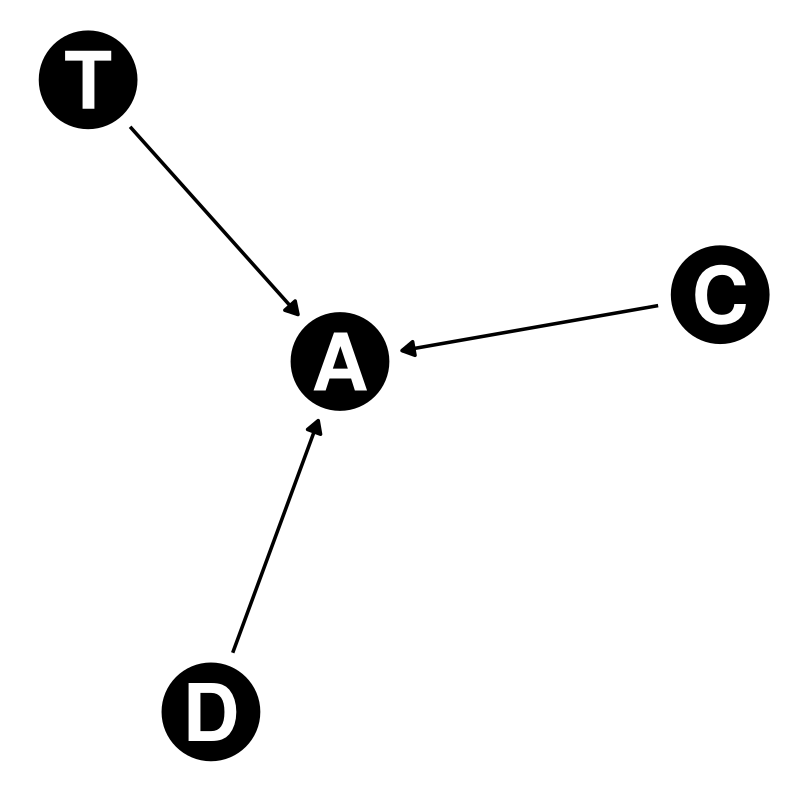
\includegraphics[width=0.40\textwidth]{../analysis/figs/dag_non_canonical_agreement.png}
\end{center}

% \noindent The three main factors previously shown to correlate to case attraction:
% \begin{compactitem}
% 	\item Copular infinitives imply a different domain of agreement, as they
% 		select different predication classes;
% 	\item Main verbs with semantic modality imply a different type of controller,
% 		as they have higher subjecthood;
% 	\item Word order and distance imply different status for the target, as
% 		targets more to the left of the sentence are both structurally closer to the
% 		controller and have a higher communicative function.
% \end{compactitem}
%
\paragraph{Copular infinitives:} proposed in by \textcite{KG}

% \noindent Copular infinitives my affect agreement by two paths:
% \begin{compactitem}
% 	\item directly: they filter the possible relations between controller and
% 		target, as those are now more likely in primary predication, rather than
% 		secondary or appositive relation.
% 	\item indirectly: by filtering the class of predication, it delimits the
% 		option of target, making it more likely that they are nouns or adjectives,
% 		rather than participles.
% \end{compactitem}
% Both would affect attraction by means of the 
% Agreement Hierarchy
% (\cite{Corbett1979}) and Predicate Hierarchy (\cite{Comrie1975}), combined into
% the Agreement and Predicate Hierarchy

\ex. Agreement and Predicate Hierarchies~(\cite[233]{Corbett2006}):\\
\begin{tikzpicture}[baseline=0pt]
    \node (attr) at (0, 0) {Attributive};
    \node (pred) at (2.5, 0) {Predicative};
    \node (predv) at (2.9, -0.4) {Verb};
    \node (predp) at (3.5, 1) {Participle};
    \node (preda) at (5, 2) {Adjective};
    \node (predn) at (7, 2.5) {Noun};
    \node (relp) at (5.6, 0) {Relative Pronoun};
    \node (perp) at (9.1, 0) {Personal Pronoun};
    \node (less) at (0, -1) {-};
    \node (plus) at (9.1, -1) {+};
    \draw[->, thick] (attr) to (pred);
    \draw[->, thick] (pred) to (relp);
    \draw[->, thick] (relp) to (perp);
    \draw[->, thick] (pred) to (predp);
    \draw[->, thick] (predp) to (preda);
    \draw[->, thick] (preda) to (predn);
    \draw[->] (less) to (plus);
    \draw[->] (plus) to (less);
    \node at (4.5, -1.5) {Likelihood of agreement with semantic justification};
\end{tikzpicture}


\paragraph{Impersonal verbs:} see~\textcite{Humbert1945}

% \textbf{Issue:} δοκέω has a rather low number of examples attesting
% attraction.

\paragraph{Verbs with modal semantics:} verbs such as ἐξαρκεῖ and ἔξεστί have higher
probability to display case attraction (\cite{Geraldes2020,Geraldes2023}).

% \noindent They do not assign thematic role to the controller, as
% in~\ref{gloss:mod}

\ex.\label{gloss:mod} ἀλλ᾽ ἐξαρκῇ σοι τὰ ἔργα αὐτῶν ὁρῶντι σέβεσθαι καὶ τιμᾶν τοὺς θεούς.\\
But it is enough for you to look at these deeds and respect the gods. 
(Xen.\ \emph{Mem.} 4.3.13)



% \begin{compactitem}
% 	\item If the matrix verb is a verb of order or advice, the oblique object has
% 		the thematic role of \textbf{Recipient}
% 	\item If the matrix verb is δοκέω, the oblique object has the thematic role of
% 		\textbf{Experiencer}
% 	\item If the matrix verb is a verb with modal semantics, the oblique object
% 		has the thematic role of either: \textbf{Experiencer} if the infinitive is a
% 		copula or a passive; or \textbf{Agent}.
% \end{compactitem}
%
% The effect of Copula flows through the Thematic role, see~\autoref{fig:dag_b}
%

\paragraph{Authorship and dialect:} \textcite{Geraldes2020,Geraldes2023} shows
that authors use verbs of modal semantic more often in philosophical dialogues.

% \noindent This may cause non\hyp{}causal effects to bias the estimated effects
% of Thematic Role and Copula, by means of the backdoor criterion
% (\cite{Pearl2009}).
% The model must account for Authorship, Genre and Dialect. See~\autoref{fig:dag_c}
% Consequences:
% \begin{compactitem}
% \item to estimate the direct effect of \textbf{Th}ematic role, we must control
% for \textbf{Cop}ula and either by \textbf{Genre} or \textbf{Auth}orship;
% \item to estimate the direct effect of \textbf{Cop}ula, we must control for
	% \textbf{P}art \textbf{o}f \textbf{S}peech, \textbf{Th}ematic role, and either
	% by \textbf{Genre} or \textbf{Auth}orship;
% \item to estimate the direct effect of \textbf{Dia}lect, we must control for
	% \textbf{Auth}orship;
% \item to estimate the direct effect of \textbf{Auth}orship, we must control for
	% \textbf{Dia}lect and by either \textbf{Genre} or \textbf{Cop}ula and
	% \textbf{Th}ematic role.
% \end{compactitem}


\paragraph{Word order and Distance:} longer distances diminish the likelihood of
case attraction. Targets preceding the controller seem to
seem to demand case attraction in examples such as~\ref{gloss:prec}.

\ex.\label{gloss:prec}ὡς \textbf{ἀγαθοῖς} τε \textbf{ὑμῖν} προσήκει εἶναι.\\
That you may be good people. (Xen.\ \emph{Anab.} 3.2.11)


% \noindent Word order is highly associated in Ancient Greek communicative
% function, see \textcite{Dik1995,Dik2007}, \textcite{Matic2003}, and \textcite{Allan2012}.
%
\paragraph{Word order and communicative function:} Word Order is not 1-1
equivalent to focus, topic and any other communicative function. It makes an
element more likely to be more topical or a focus, but there are unobserved
features.% See~\autoref{fig:dag_d}.

% As the effect of Word Order also flows through unobserved features of the
% target, it is not possible to estimate its direct effect statistically.

\paragraph{Distance flows from Word Order:} Since distance depends on word
order, we can only estimate the direct effect by controlling for Word Order.


\begin{figure}[hbt]
	\centering
	\begin{minipage}{.45\textwidth}
	\begin{center}
	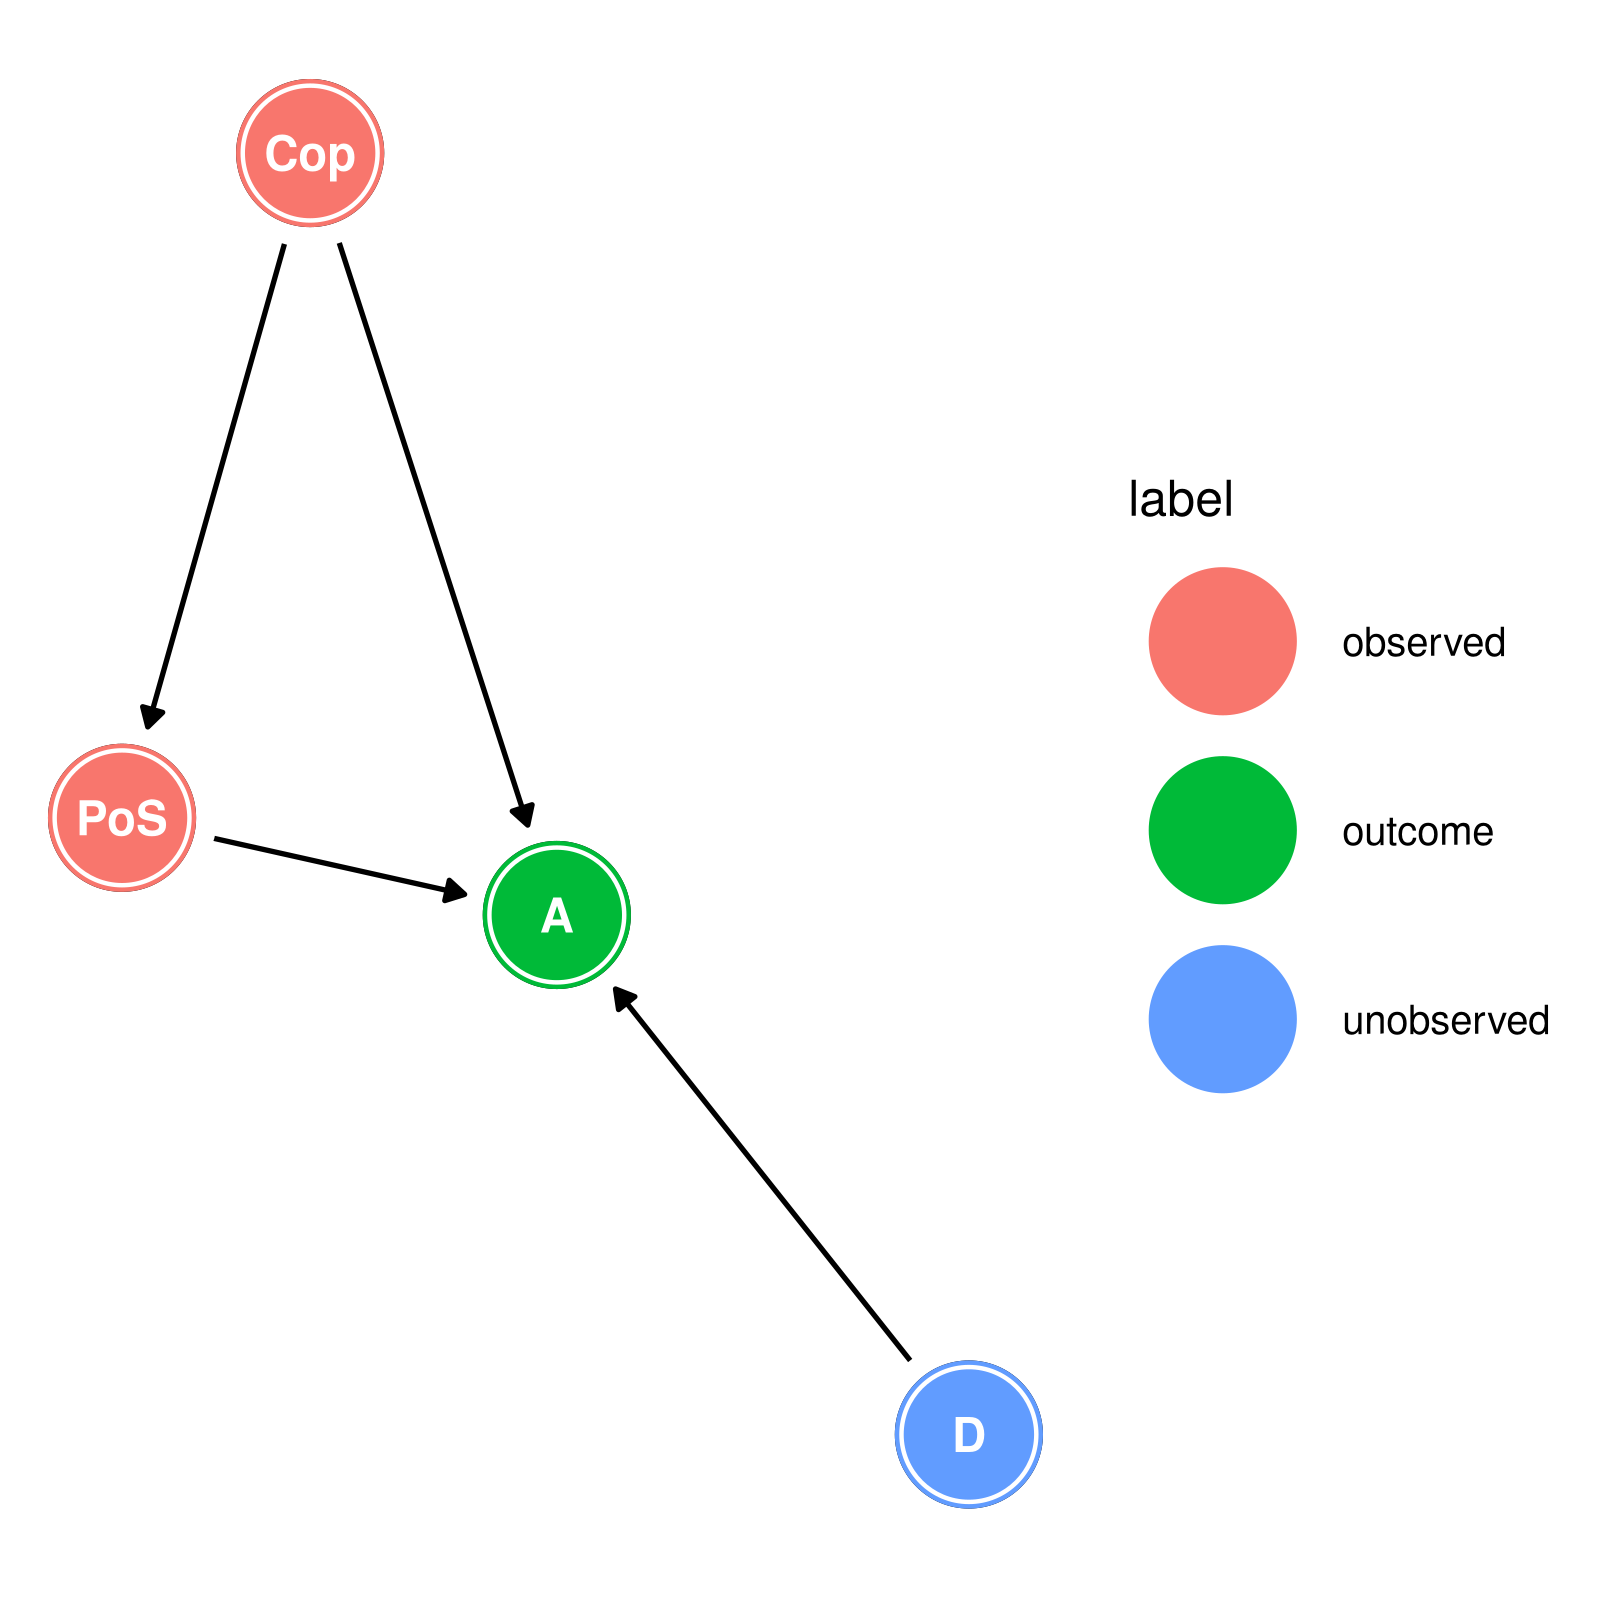
\includegraphics[width=\linewidth]{../analysis/figs/dag_a.png}
	\end{center}
	\caption{DAG with \textbf{A}ttraction, \textbf{D}omain,
	\textbf{P}art \textbf{o}f \textbf{S}preech and \textbf{C}opula}\label{fig:dag_a}
\end{minipage}
\hfill
	\begin{minipage}{.45\textwidth}
	\begin{center}
	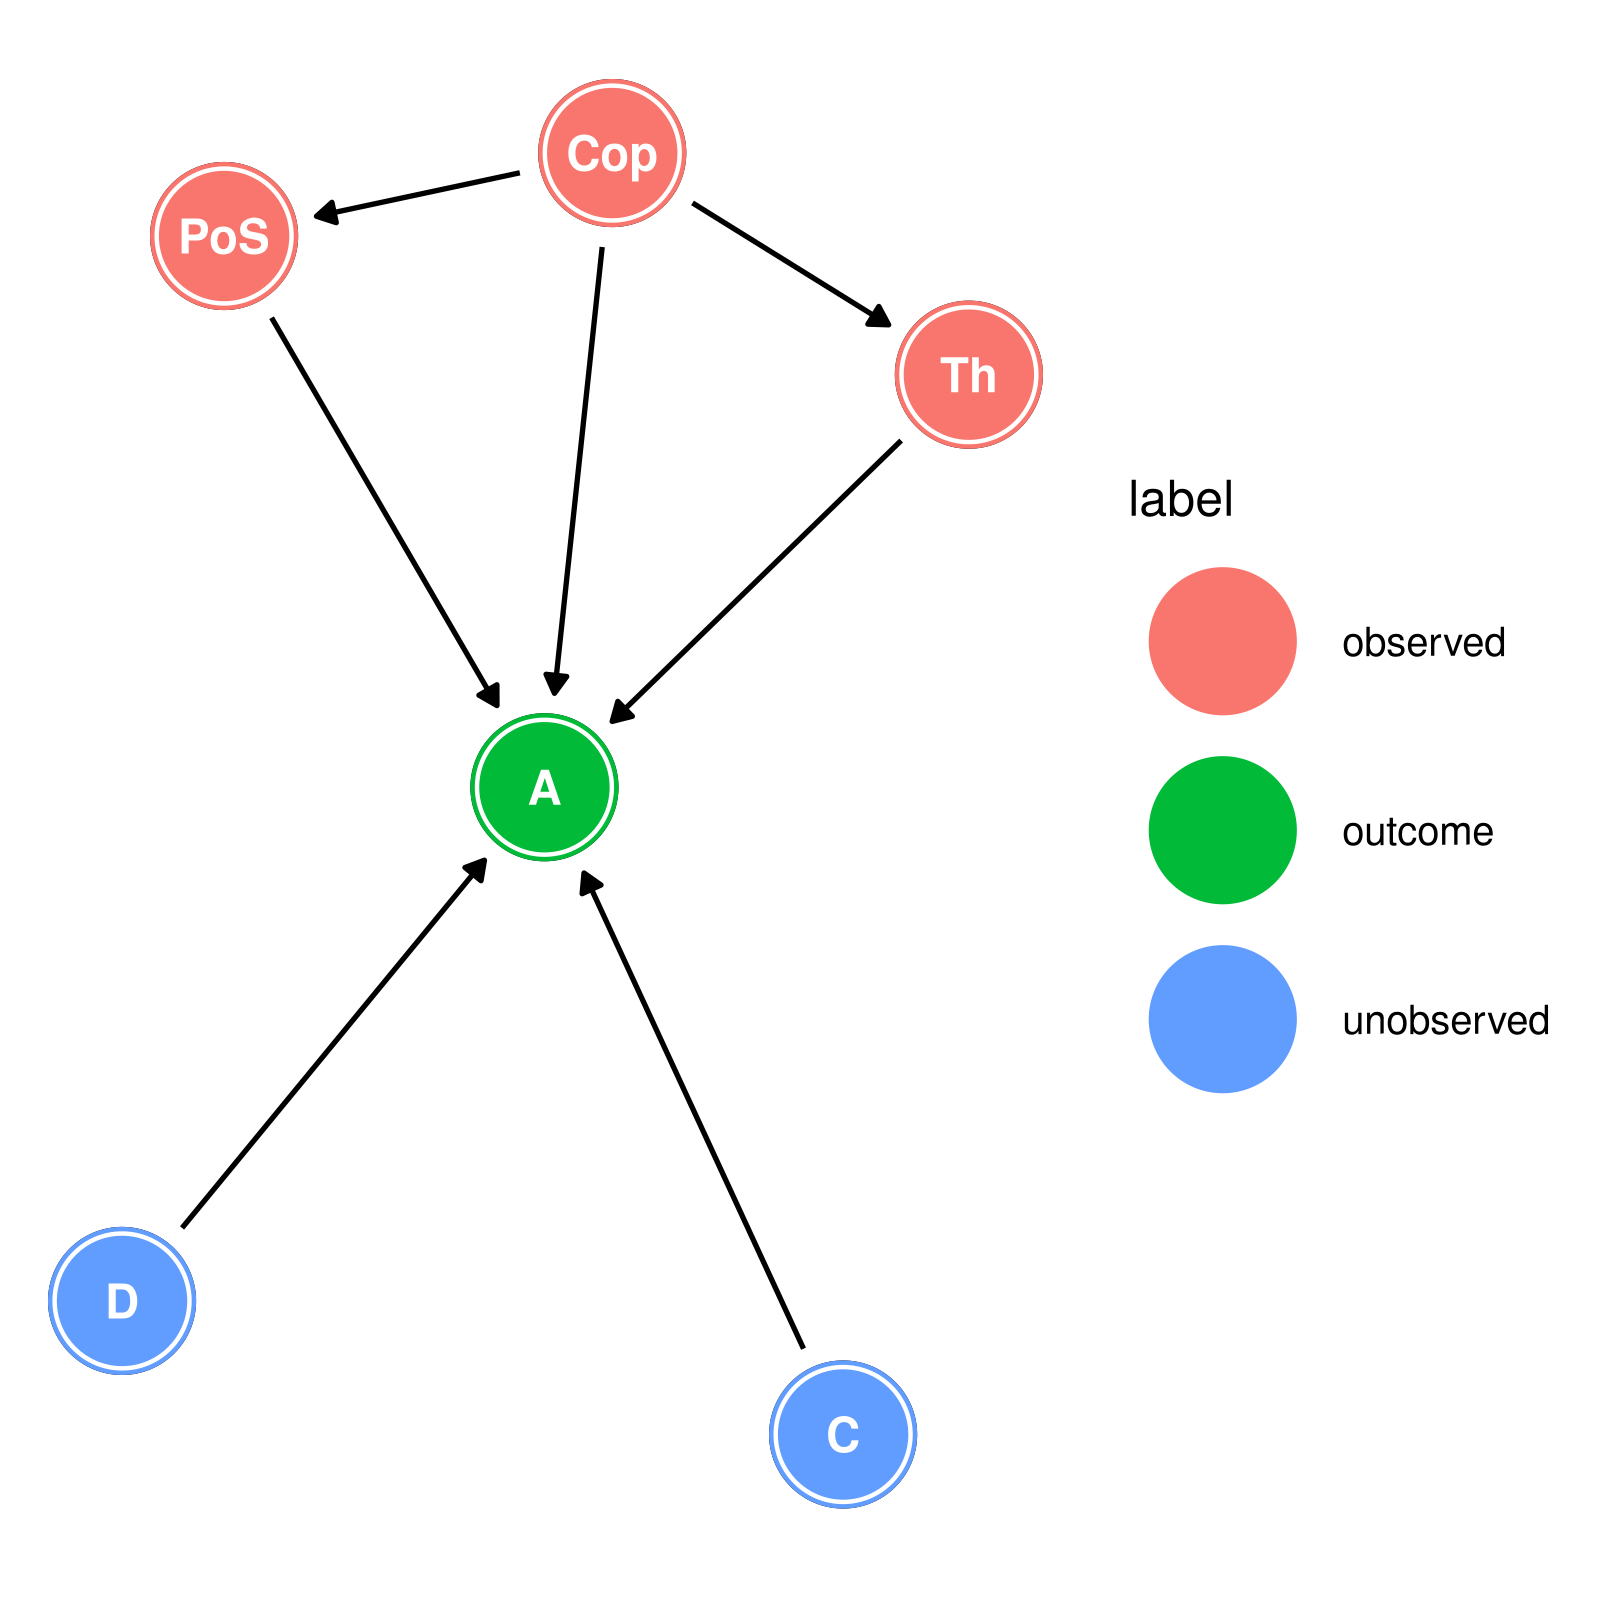
\includegraphics[width=\linewidth]{../analysis/figs/dag_b.png}
	\end{center}
	\caption{DAG with \textbf{A}ttraction, \textbf{D}omain, \textbf{C}ontroller
	\textbf{P}art \textbf{o}f \textbf{S}preech, \textbf{C}opula and
\textbf{Th}ematic role.}\label{fig:dag_b}
\end{minipage}
\end{figure}

\begin{figure}[hbt]
	\centering
	\begin{minipage}{.45\textwidth}
	\begin{center}
	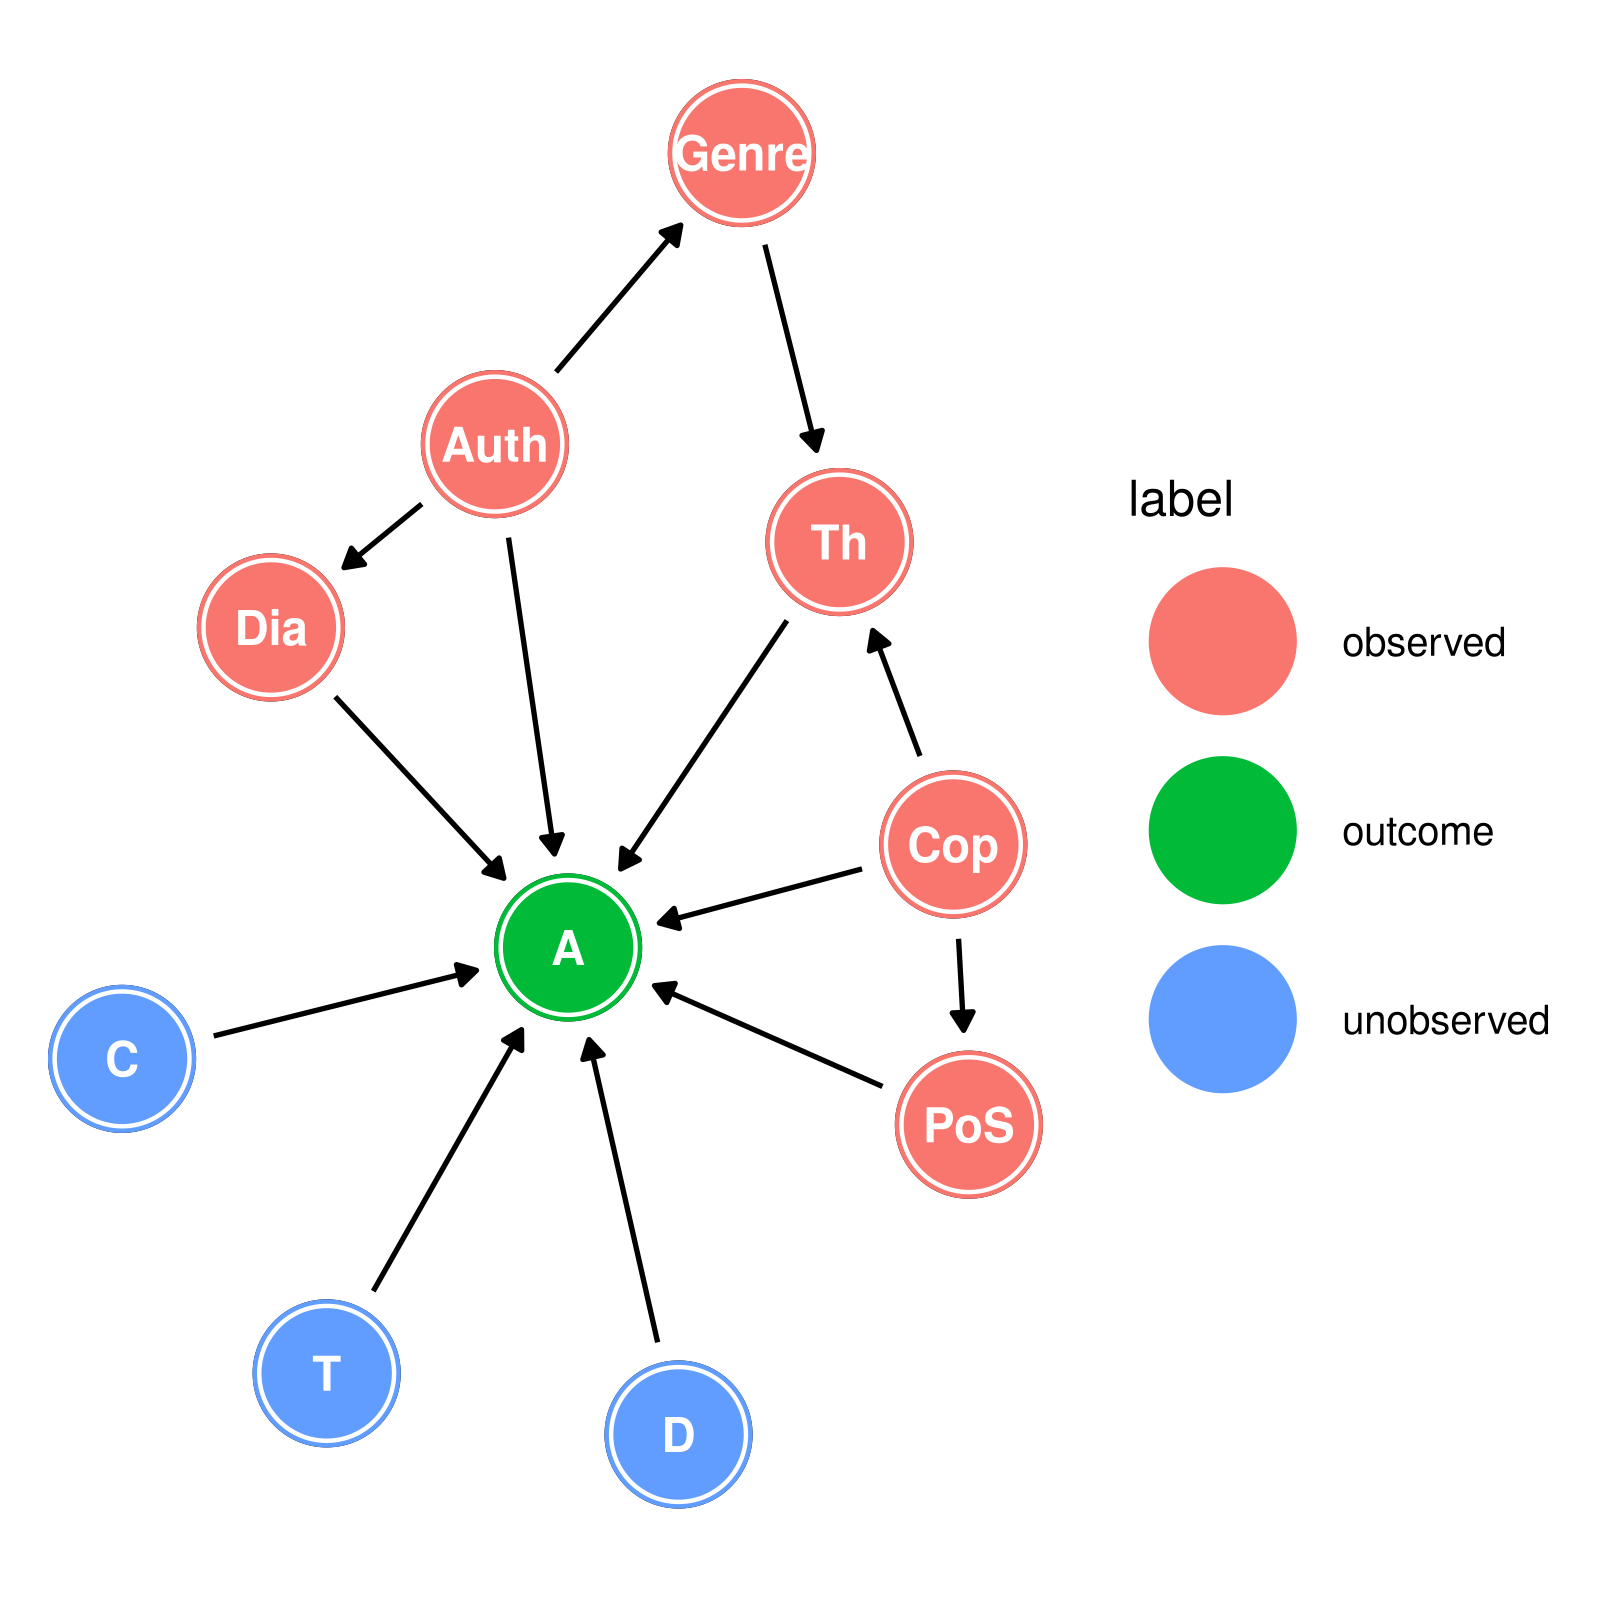
\includegraphics[width=\linewidth]{../analysis/figs/dag_c.png}
	\end{center}
	\caption{DAG with \textbf{A}ttraction, \textbf{D}omain, \textbf{C}ontroller
	\textbf{P}art \textbf{o}f \textbf{S}preech, \textbf{C}opula,
	\textbf{Th}ematic role, \textbf{Auth}orship, \textbf{Genre}, and
	\textbf{Dia}lect.
}\label{fig:dag_c}
\end{minipage}
\hfill
	\begin{minipage}{.45\textwidth}
	\begin{center}
	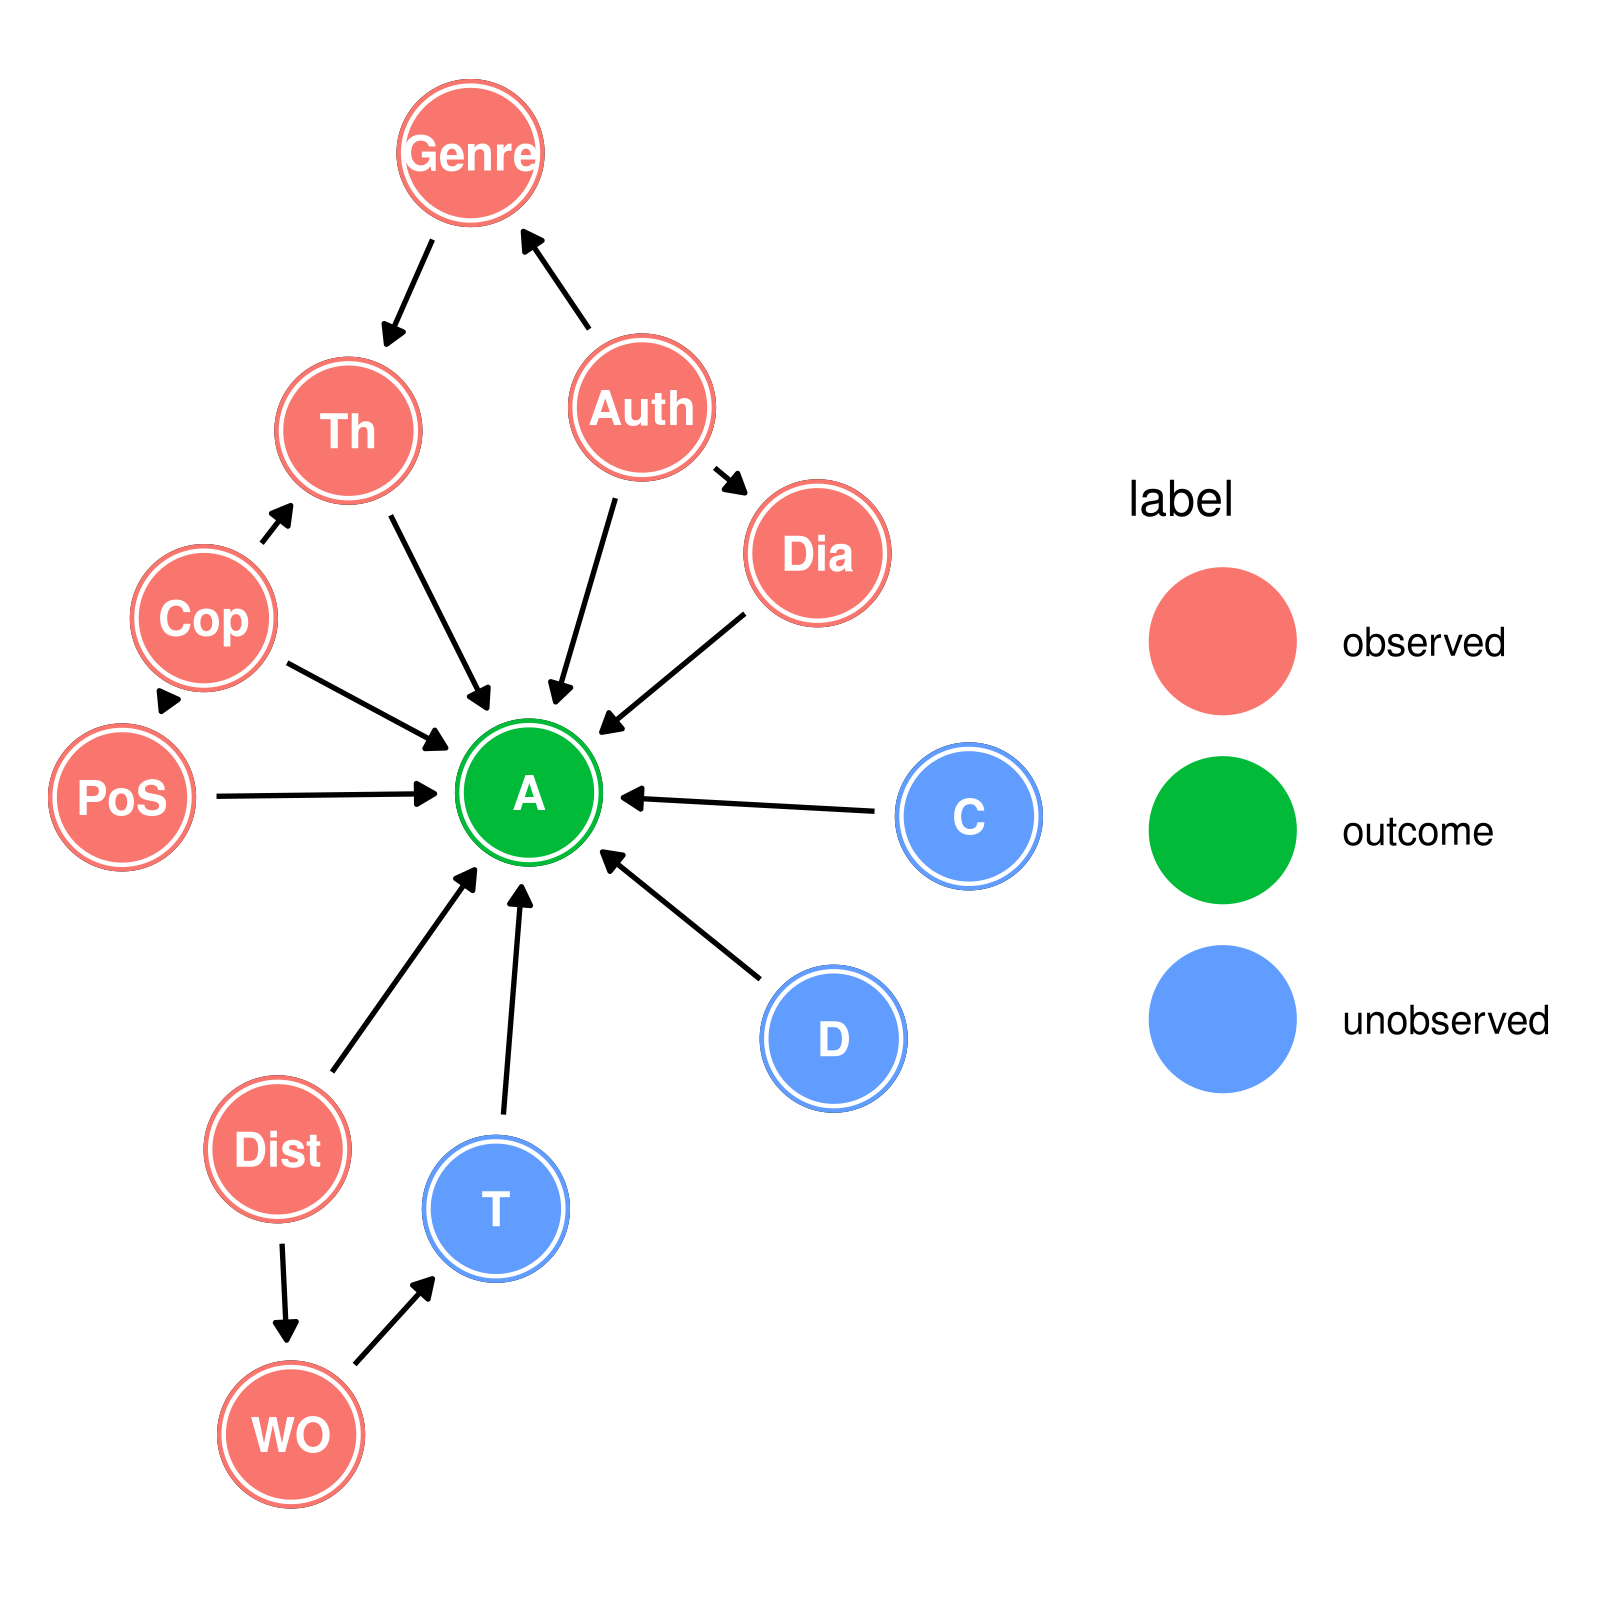
\includegraphics[width=\linewidth]{../analysis/figs/dag_d.png}
	\end{center}
	\caption{DAG with \textbf{A}ttraction, \textbf{D}omain, \textbf{C}ontroller,
		\textbf{T}arget,
	\textbf{P}art \textbf{o}f \textbf{S}preech, \textbf{C}opula,
	\textbf{Th}ematic role, \textbf{Auth}orship, \textbf{Genre}, 
	\textbf{Dia}lect, \textbf{Dist}ance, and \textbf{W}ord \textbf{O}rder.
}
\end{minipage}
\end{figure}


\clearpage

\paragraph{Final causal model:}

	\begin{center}
	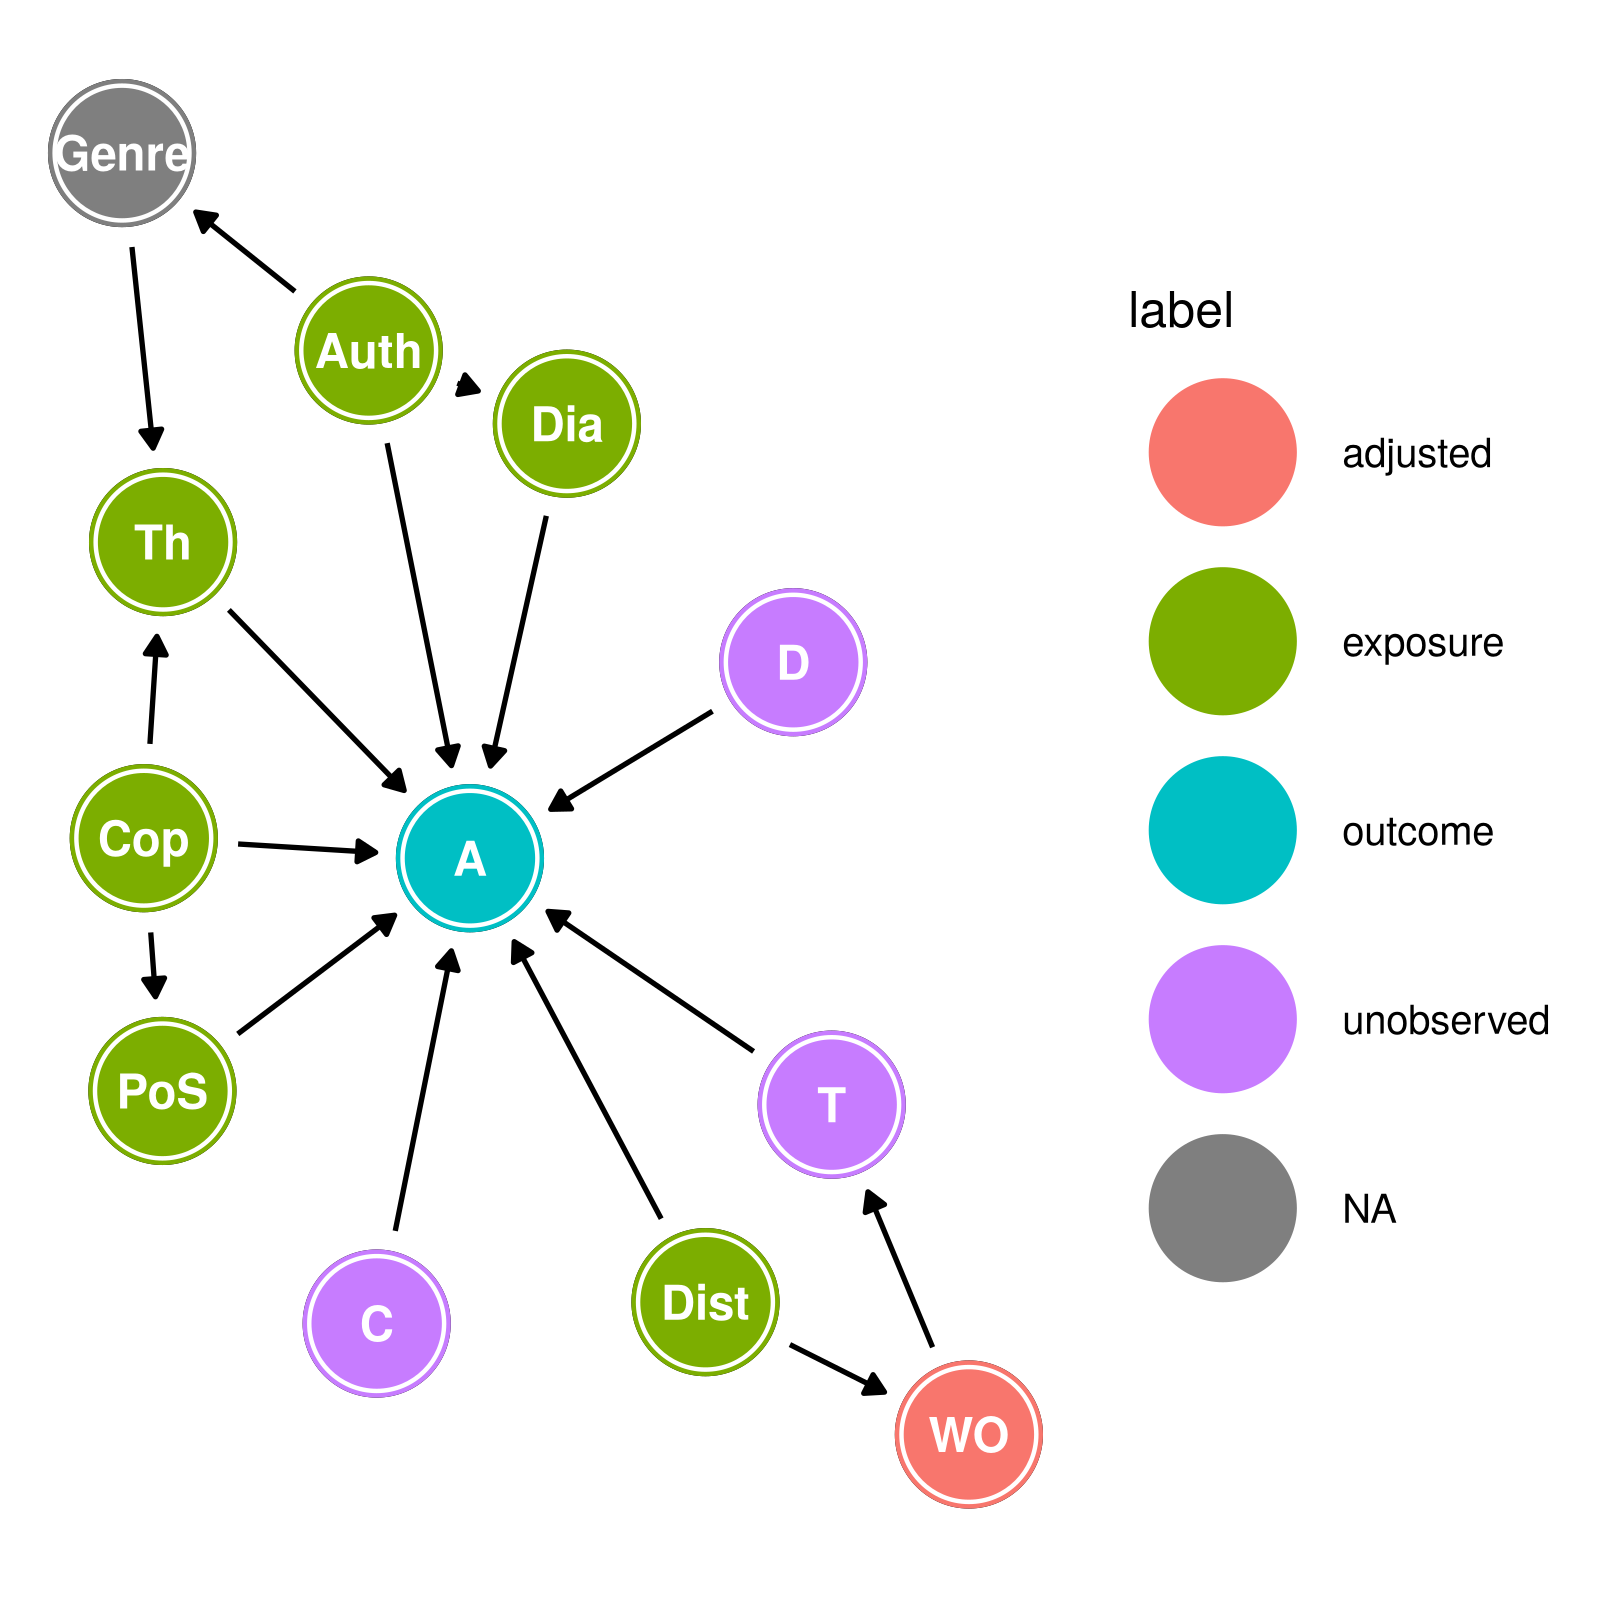
\includegraphics[width=0.75\linewidth]{../analysis/figs/dag_e.png}
	\end{center}

	\noindent Adjustment set: $WO$



\paragraph{Generalized linear model:}
\begin{align*}
	\text{A} &\sim \text{Bernoulli}(p_i)\\
	\text{logit}(p_i) &= \alpha + 
	\beta_{\text{Cop}}\text{Cop}_i + 
	\beta_{\text{Dist}}\text{Dist}_i + \beta_{\text{WO}} \text{Prec}_i \\&+
	\beta_{\text{PoS}}\sum^{PoS_{i}-1}_{j=0}{\delta_{j_{\text{PoS}}}} + \beta_{\text{Th}}\sum^{Th_{i}-1}_{j=0}{\delta_{j_{\text{Th}}}} \\&+
		\beta_{\text{Auth}_{i}} + \beta_{\text{Dia}_i}\\
	\alpha &\sim \text{Normal}(0, 1)\\
	\beta_{\text{Cop}}, \beta_{\text{Dist}}, \beta_{\text{Prec}} &\sim \text{Normal}(0, 1)\\
	\beta_{\text{PoS}}, \beta_{\text{Th}} &\sim \text{Normal}(0, 0.5)\\
	\delta_{\text{PoS}}, \delta_{\text{Th}} &\sim \text{Dirichlet}(2)\\
	\beta_{\text{Auth}} &= z_{\text{Auth}}*\sigma_{\text{Auth}}\\
	\beta_{\text{Dia}} &= z_{\text{Dia}}*\sigma_{\text{Dia}}\\
	z_{\text{Auth}}, z_{\text{Dia}} &\sim \text{Normal}(0,1)\\
	\sigma_{\text{Auth}}, \sigma_{\text{Dia}} &\sim \text{Exponential}(1)
\end{align*}

\paragraph{Copula and Distance} % (fold)

\begin{center}
	
\begin{tabular}[t]{lrrrrr}
\toprule
Effect & mean & sd & 5.5\% & 94.5\% & rhat\\
\midrule
$\beta_{\text{Copula}}$ & 2.03 & 0.39 & 1.42 & 2.66 & 1\\
$\beta_{\text{Dist}}$ & -0.22 & 0.04 & -0.29 & -0.16 & 1\\
\bottomrule
\end{tabular}

\end{center}

\begin{figure}[!h]
\centering
\begin{minipage}{.48\textwidth}
  \centering
  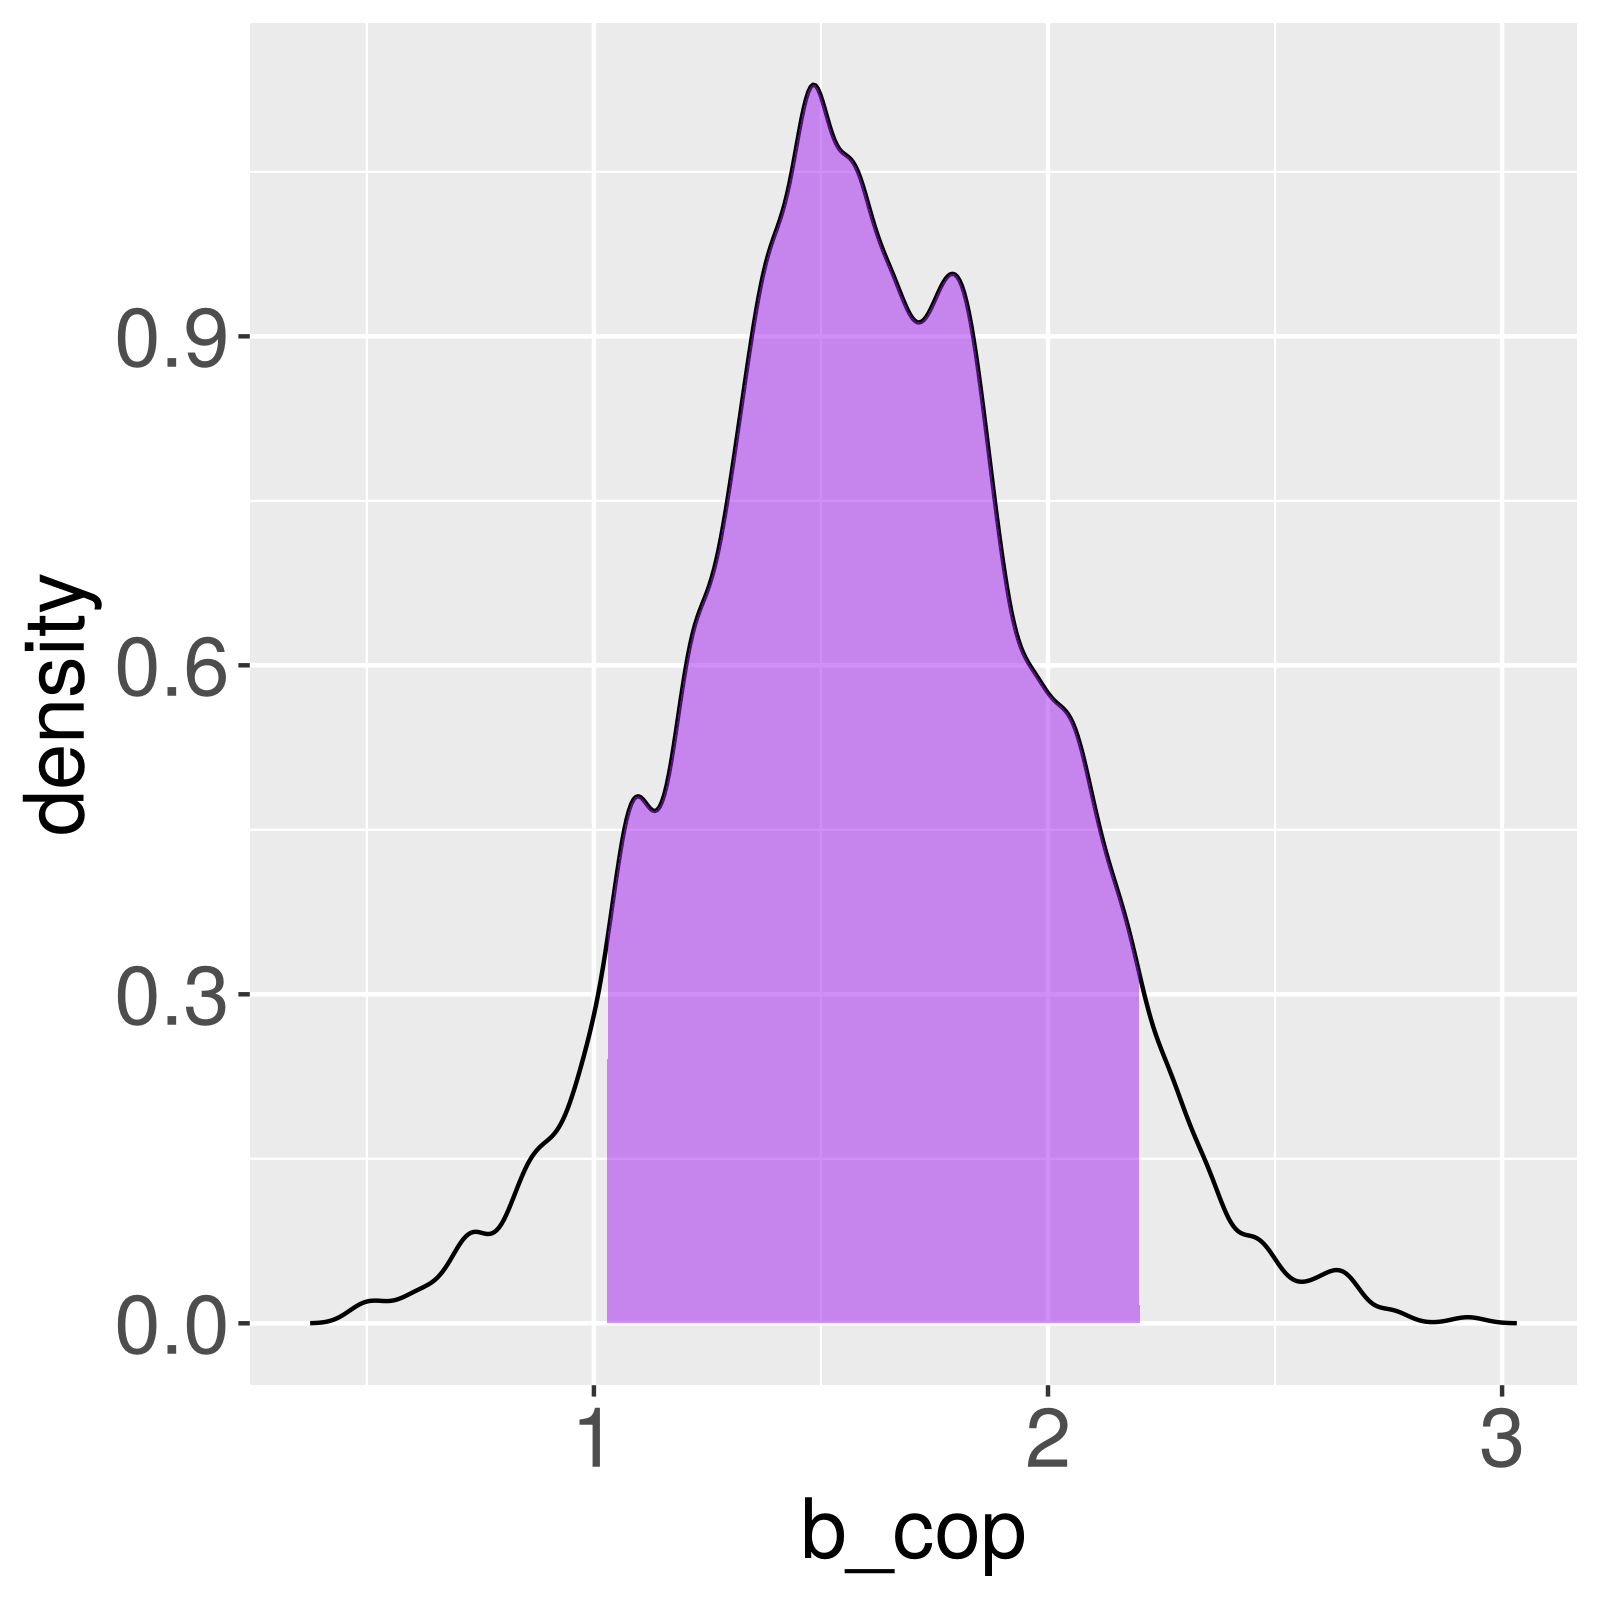
\includegraphics[width=\linewidth]{../analysis/figs/posterior_b_copula.png}
	\captionof{figure}{Posterior distribution of $\beta_\text{Cop}$ with the 89\%
	Highest Posterior Density Interval.}
\end{minipage}%
\hfill
\begin{minipage}{.48\textwidth}
  \centering
  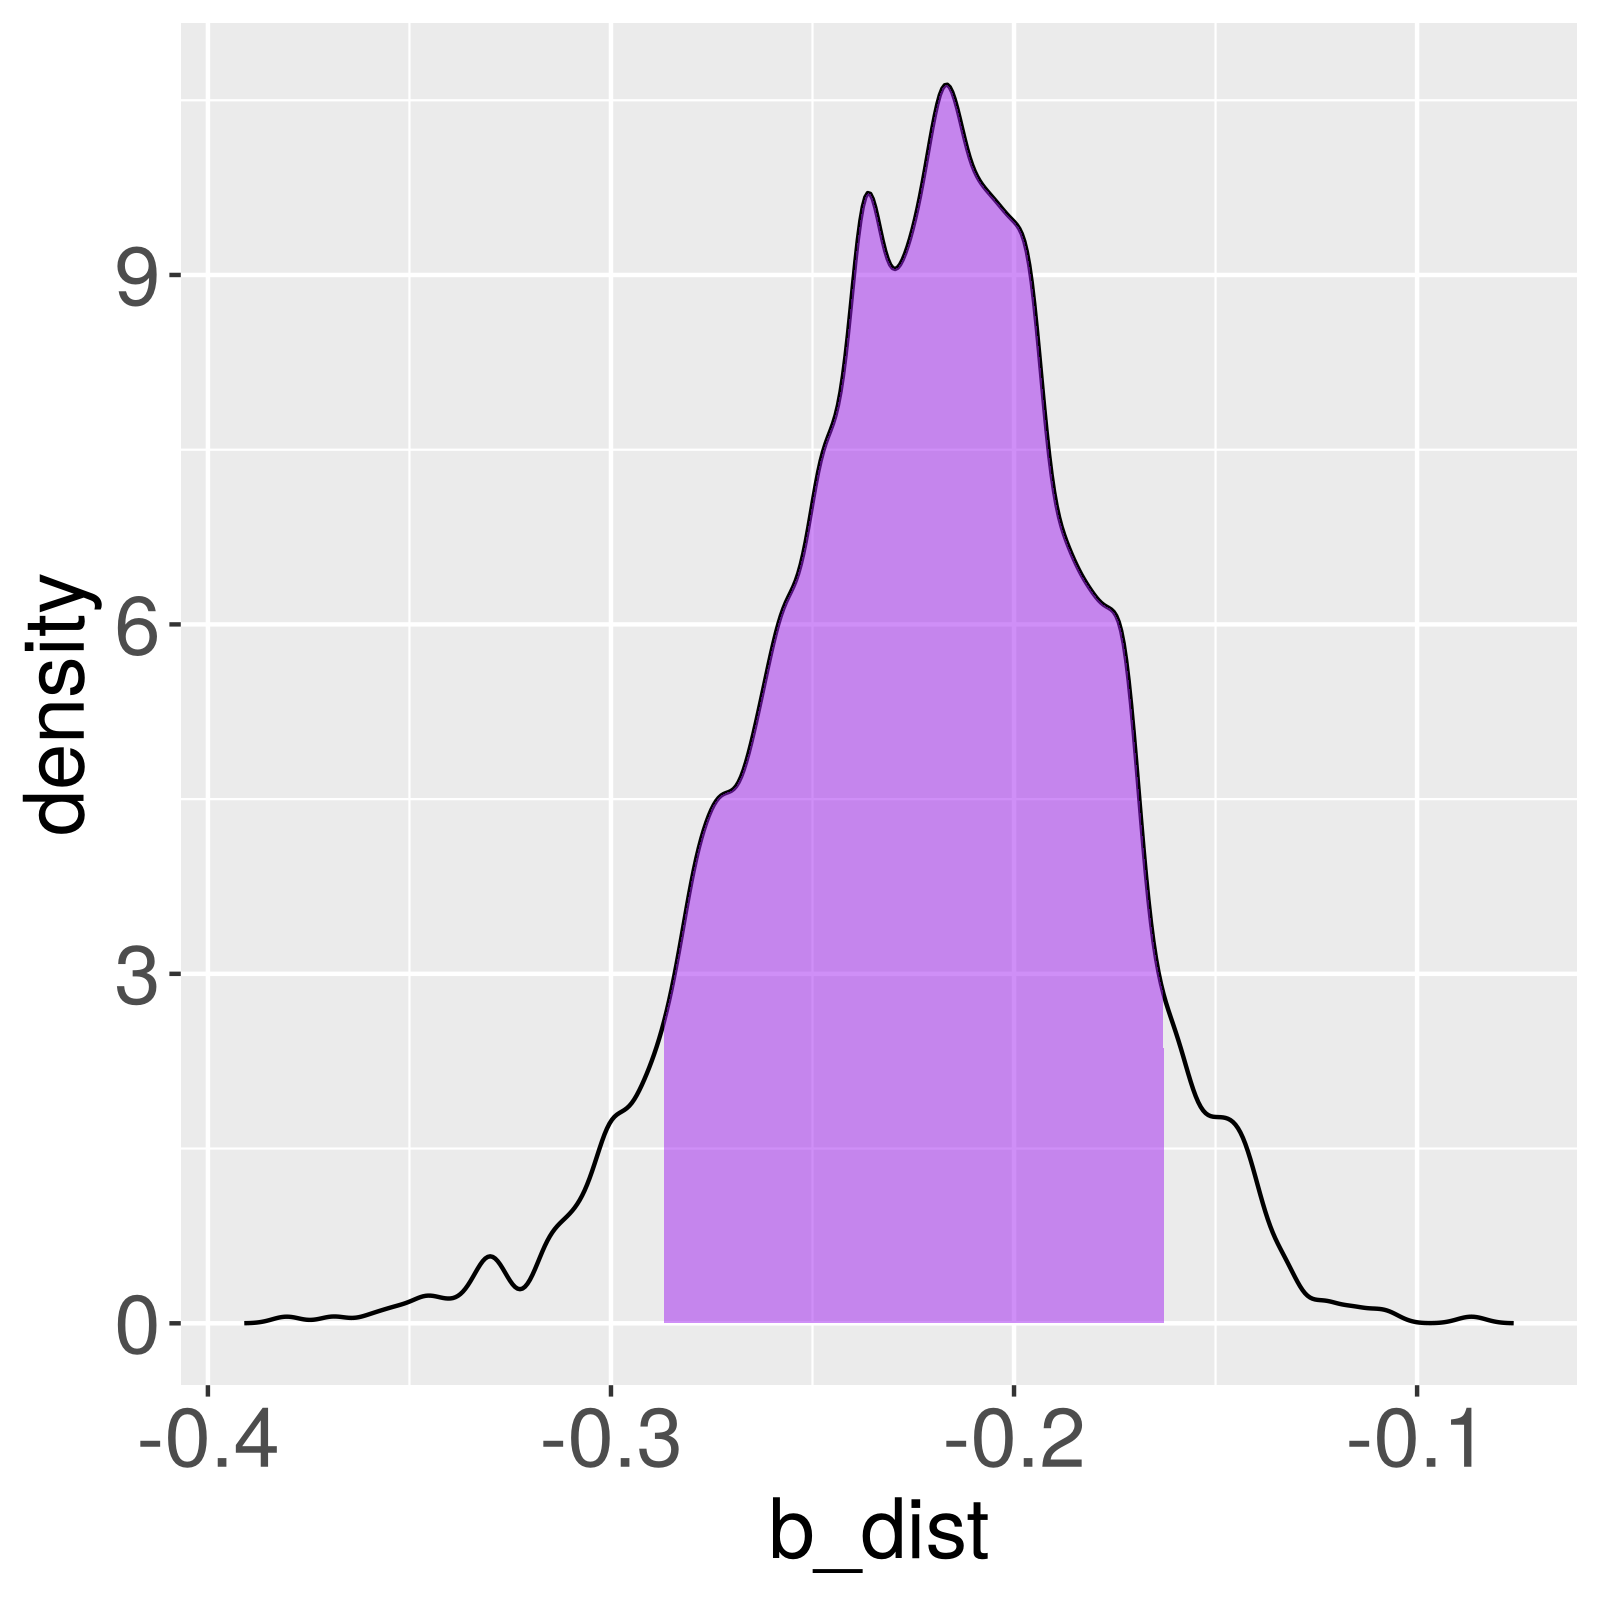
\includegraphics[width=\linewidth]{../analysis/figs/posterior_b_dist.png}
	\captionof{figure}{Posterior distribution of $\beta_\text{Dist}$ with the 89\%
	Highest Posterior Density Interval.}
\end{minipage}
\end{figure}

\paragraph{Part of Speech and the Predicate Hierarchy} % (fold)

\begin{center}
	
\begin{tabular}[t]{lrrrrr}
\toprule
Effect & mean & sd & 5.5\% & 94.5\% & rhat\\
\midrule
$\beta_{\text{PoS}}$ & 0.45 & 0.28 & 0.11 & 0.95 & 1\\
$\delta_{\text{Adj}}$ & 0.53 & 0.18 & 0.23 & 0.82 & 1\\
$\delta_{\text{Noun}}$ & 0.47 & 0.18 & 0.18 & 0.77 & 1\\
\bottomrule
\end{tabular}

	\bigskip
	
\begin{tabular}[t]{llrrrrr}
\toprule
PoS & Cummulative effect & mean & sd & 5.5\% & 94.5\% & rhat\\
\midrule
Participle & $\beta_{\text{PoS}} * 0$ & 0.00 & 0.00 & 0.00 & 0.00 & NA\\
Adjective & $\beta_{\text{PoS}} * \delta_{\text{Adj}}$ & 0.25 & 0.18 & 0.05 & 0.60 & 1\\
Noun & $\beta_{\text{PoS}} * (\delta_{\text{Adj}} + \delta_{\text{Noun}})$ & 0.45 & 0.28 & 0.11 & 0.95 & 1\\
\bottomrule
\end{tabular}

\end{center}


\begin{center}
	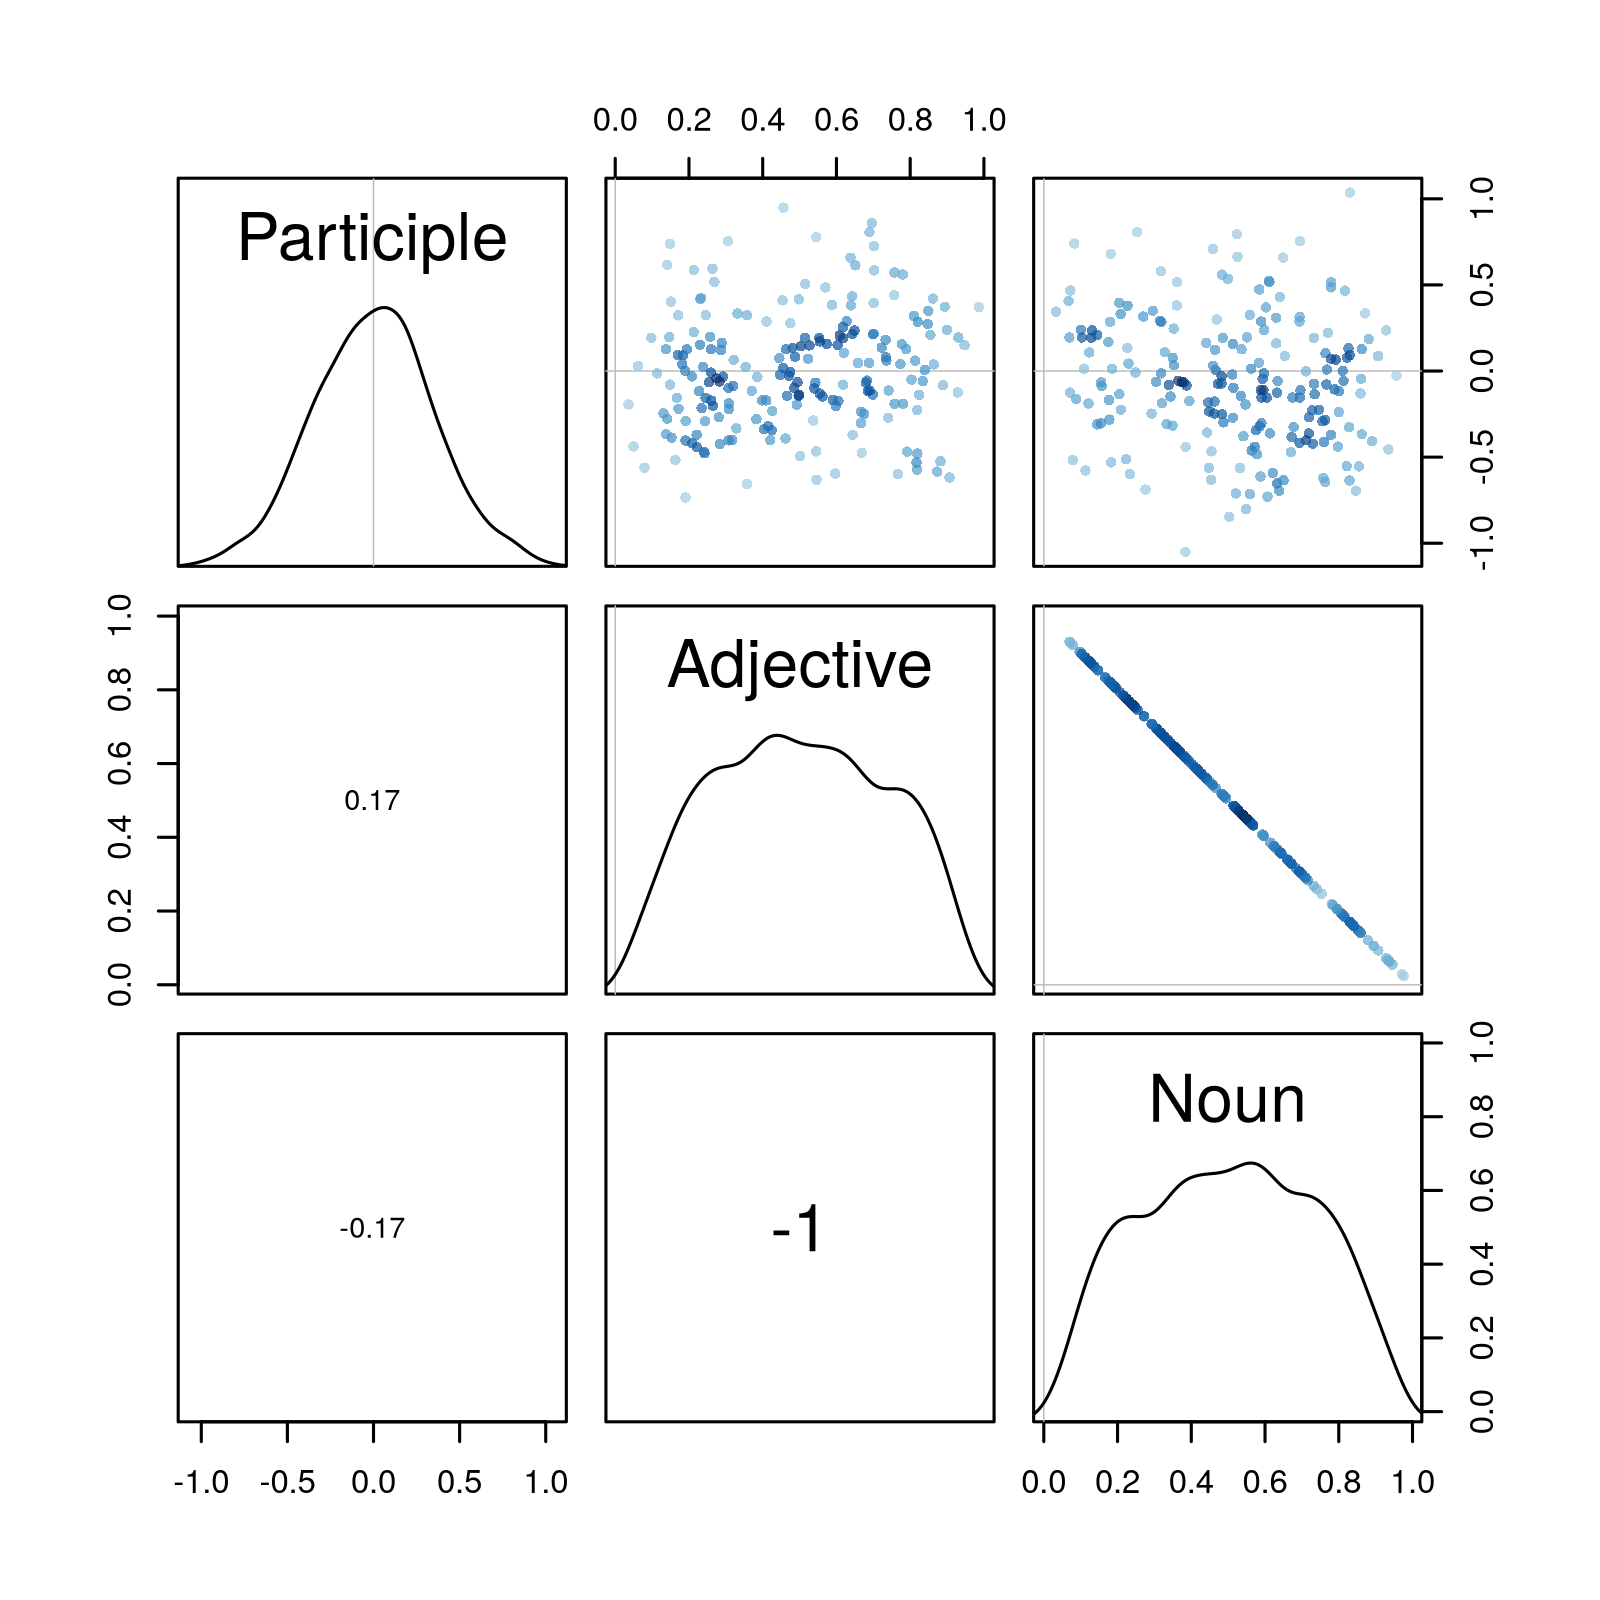
\includegraphics[width=0.70\linewidth]{../analysis/figs/model_domain_banddelta.png}
\end{center}

\paragraph{Thematic Role of the Controller} % (fold)

\begin{center}
	
\begin{tabular}[t]{lrrrrr}
\toprule
Effect & mean & sd & 5.5\% & 94.5\% & rhat\\
\midrule
$\beta_{\text{Theta}}$ & 2.47 & 0.40 & 1.84 & 3.12 & 1\\
$\delta_{\text{Exp}}$ & 0.34 & 0.11 & 0.17 & 0.51 & 1\\
$\delta_{\text{Agent}}$ & 0.66 & 0.11 & 0.49 & 0.83 & 1\\
\bottomrule
\end{tabular}

	\bigskip
	
\begin{tabular}[t]{llrrrrr}
\toprule
Theta & Cummulative effect & mean & sd & 5.5\% & 94.5\% & rhat\\
\midrule
Recipient & $\beta_{\text{Rec}}$ & 1.63 & 0.29 & 1.17 & 2.10 & 1\\
Experiencer & $\beta_{\text{Rec}} + \delta_{\text{Exp}}$ & 1.91 & 0.32 & 1.40 & 2.44 & 1\\
Agent & $\beta_{\text{Rec}} + \delta_{\text{Exp}} + \delta_{\text{Agent}}$ & 2.63 & 0.29 & 2.17 & 3.10 & 1\\
\bottomrule
\end{tabular}

\end{center}

\begin{center}
	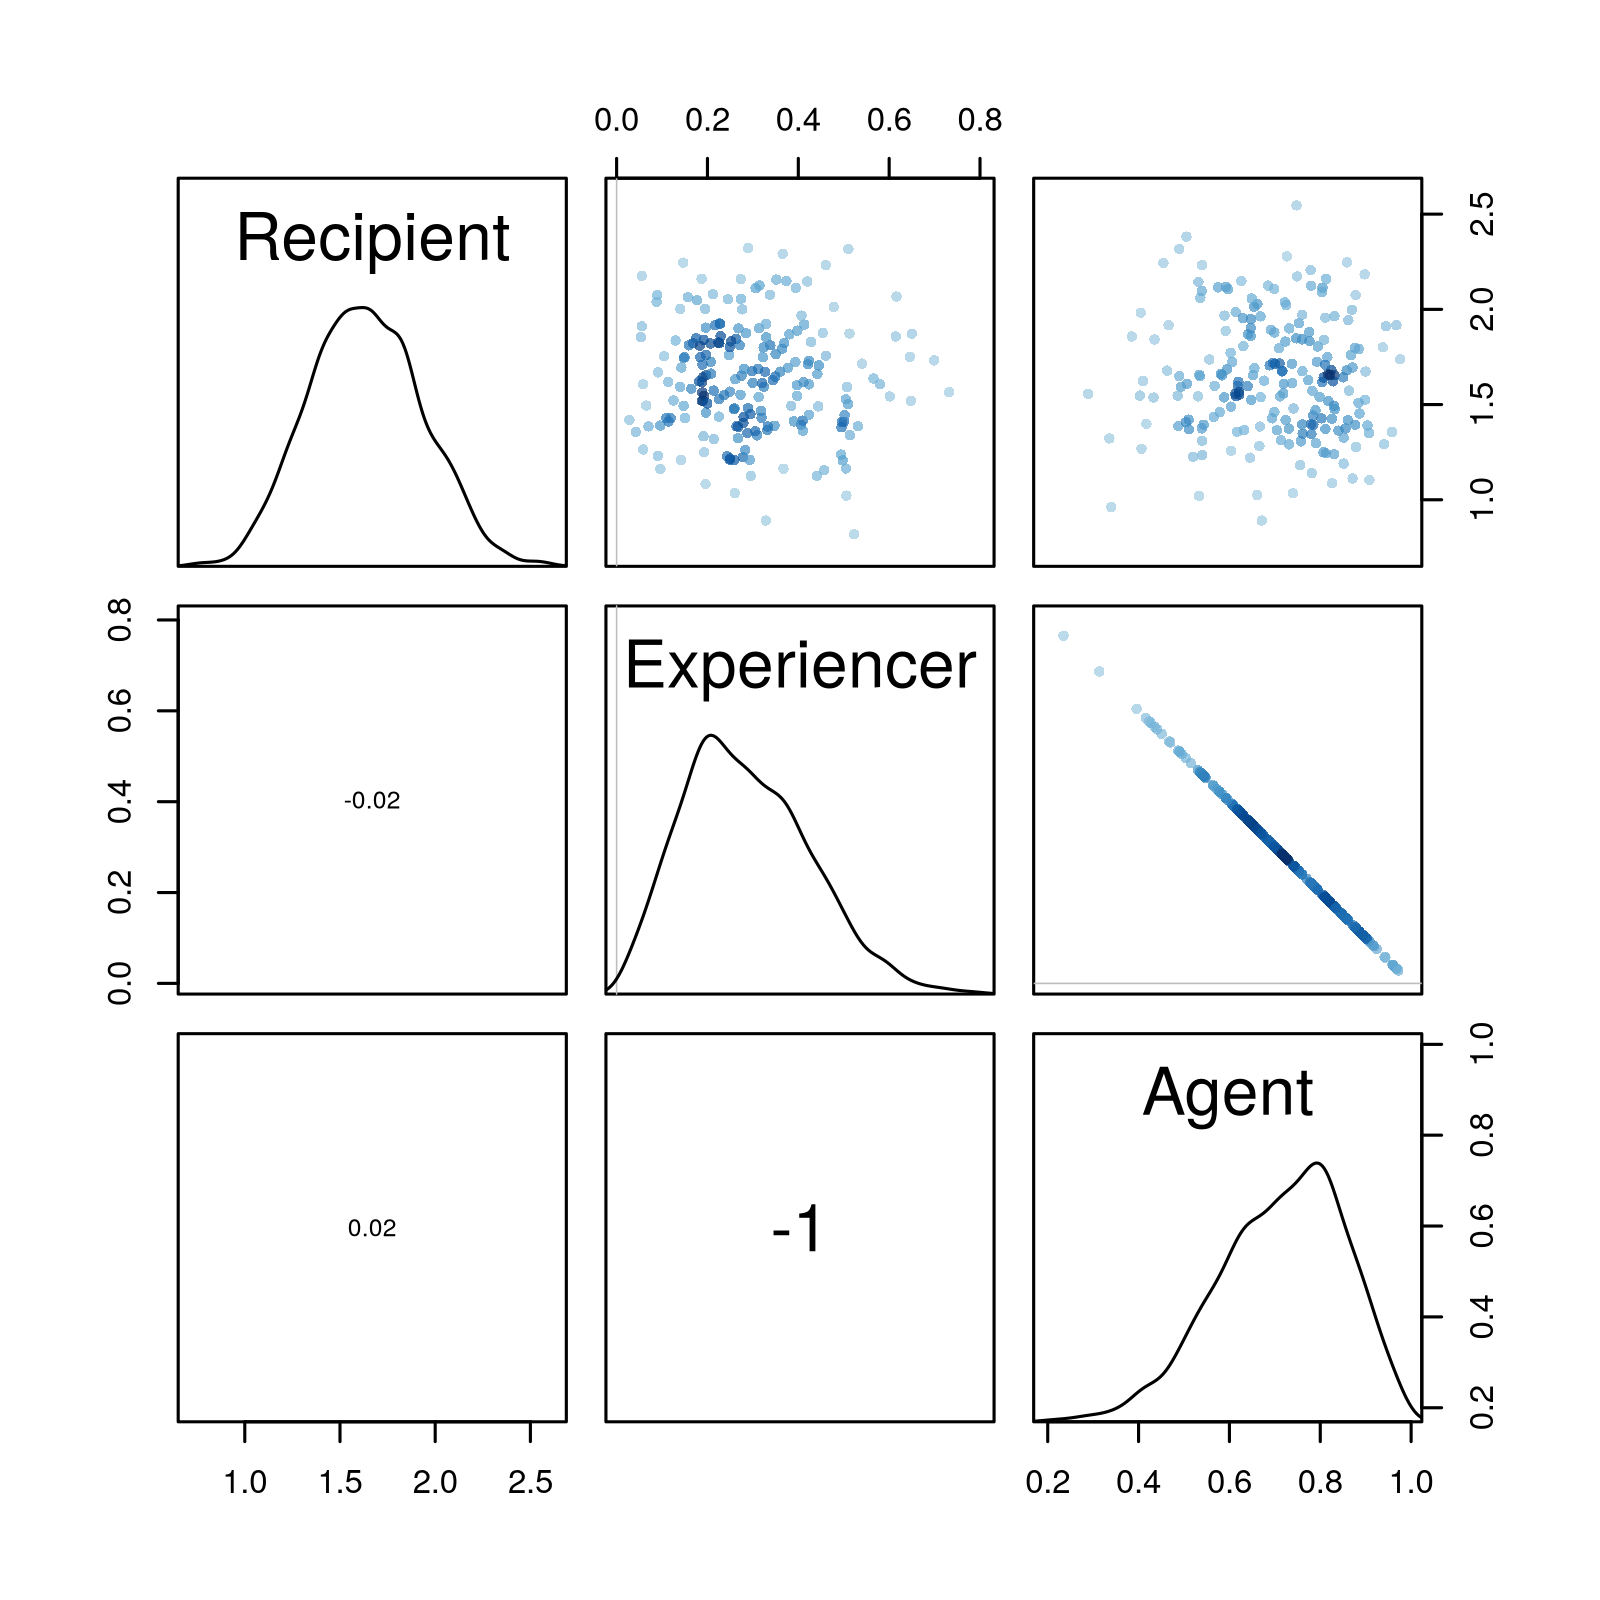
\includegraphics[width=0.75\linewidth]{../analysis/figs/model_theta_banddelta.png}
\end{center}

\paragraph{Dialect and Authorship} % (fold)

\begin{center}
	
\begin{tabular}[t]{lrrrrr}
\toprule
Effect & mean & sd & 5.5\% & 94.5\% & rhat\\
\midrule
$\beta_{\text{Attic}}$ & 0.57 & 0.73 & -0.56 & 1.74 & 1\\
$\beta_{\text{Jonic}}$ & -1.20 & 0.84 & -2.63 & -0.01 & 1\\
\bottomrule
\end{tabular}

\end{center}

\begin{figure}[!h]
\centering
  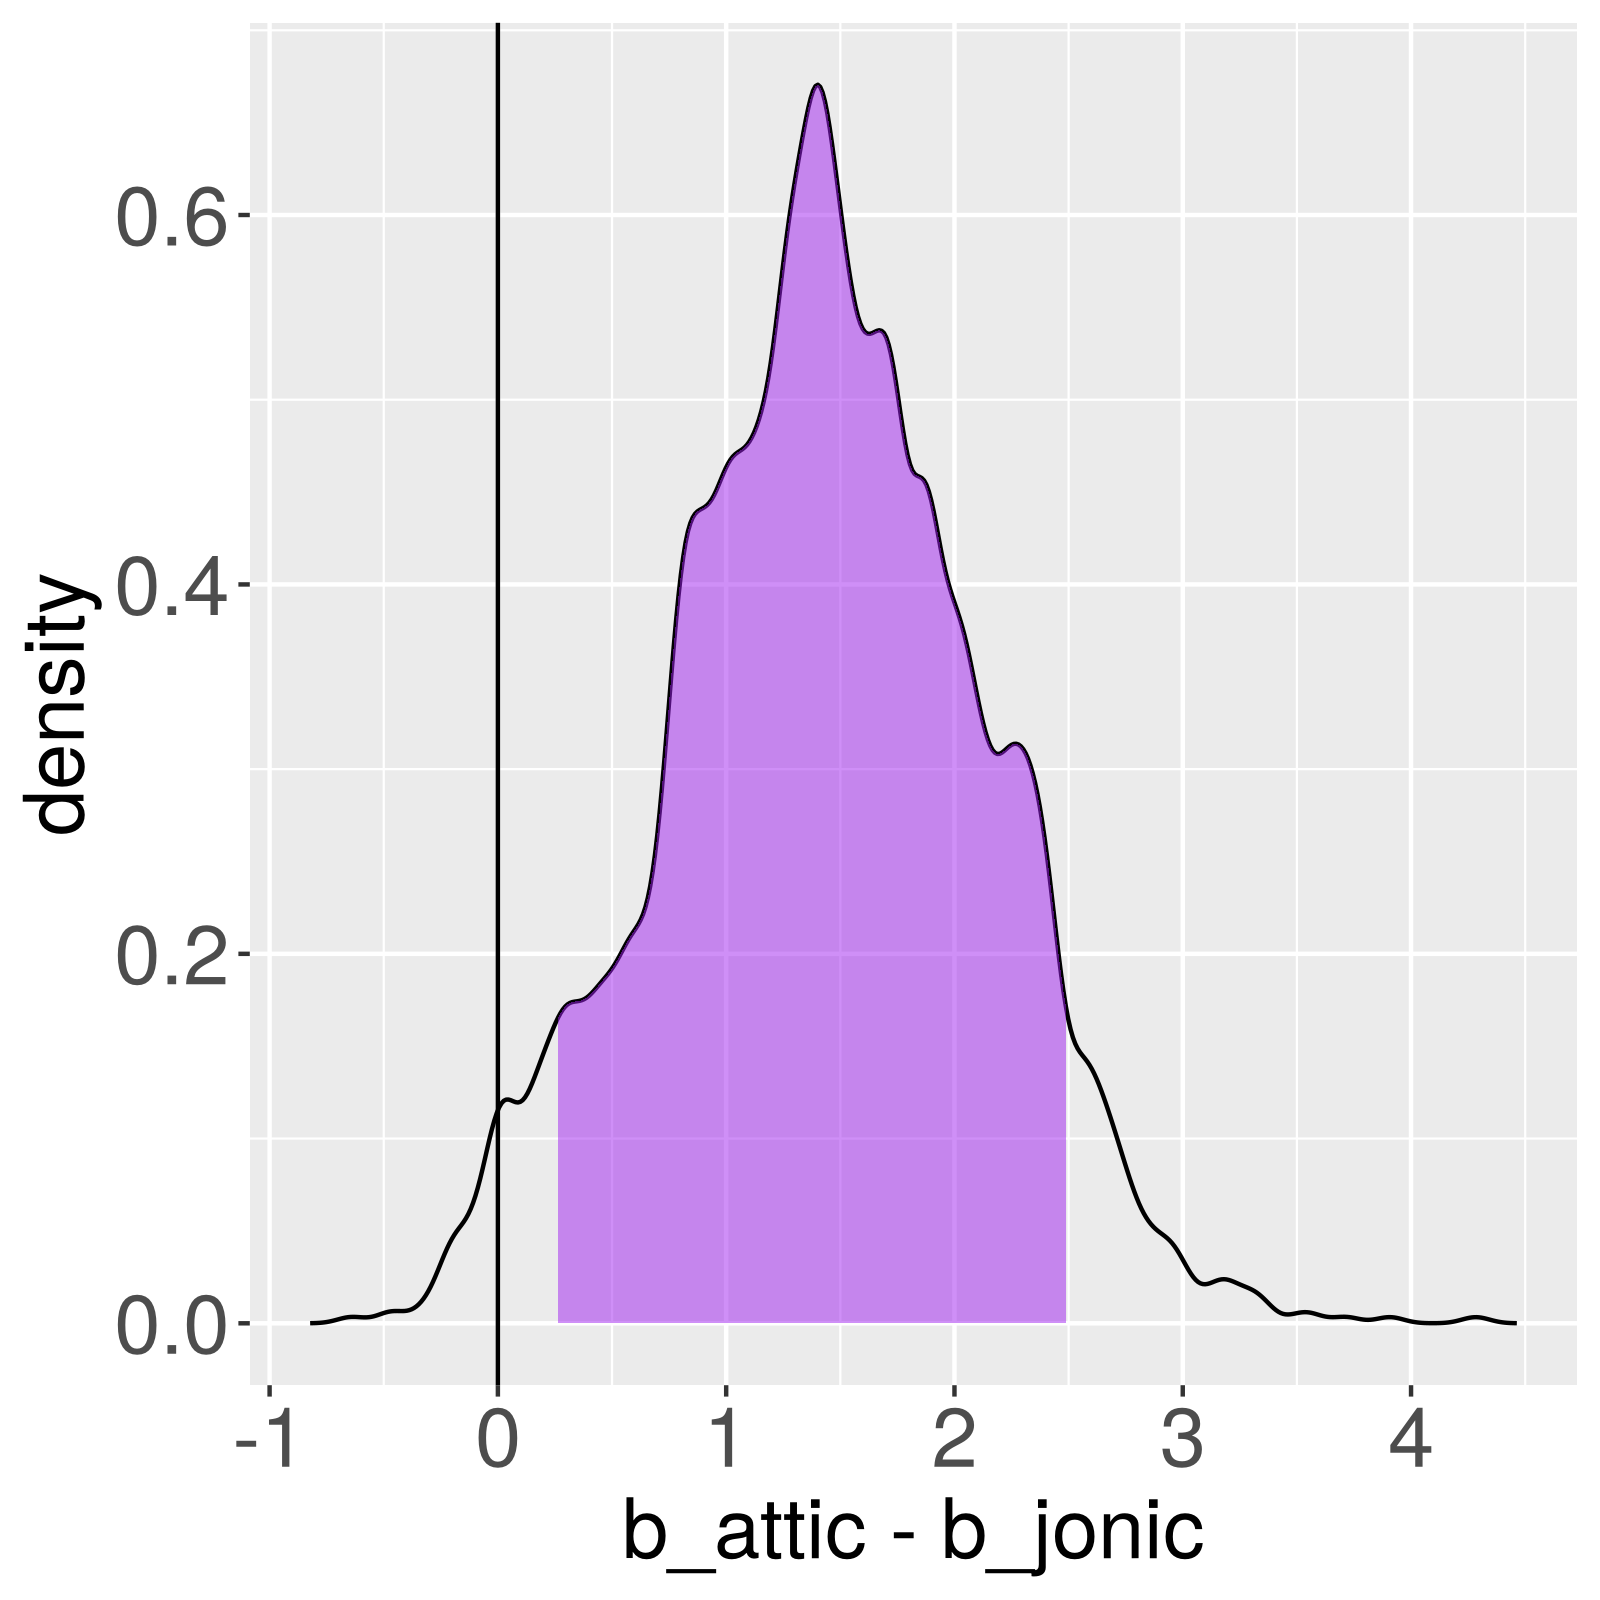
\includegraphics[width=0.5\linewidth]{../analysis/figs/posterior_diff_dia.png}
	\caption{Posterior distribution of the difference between
		$\beta_\text{Attic}$ and $\beta_\text{Jonic}$ with the 89\%
	Highest Posterior Density Interval.}
\end{figure}

\begin{center}
	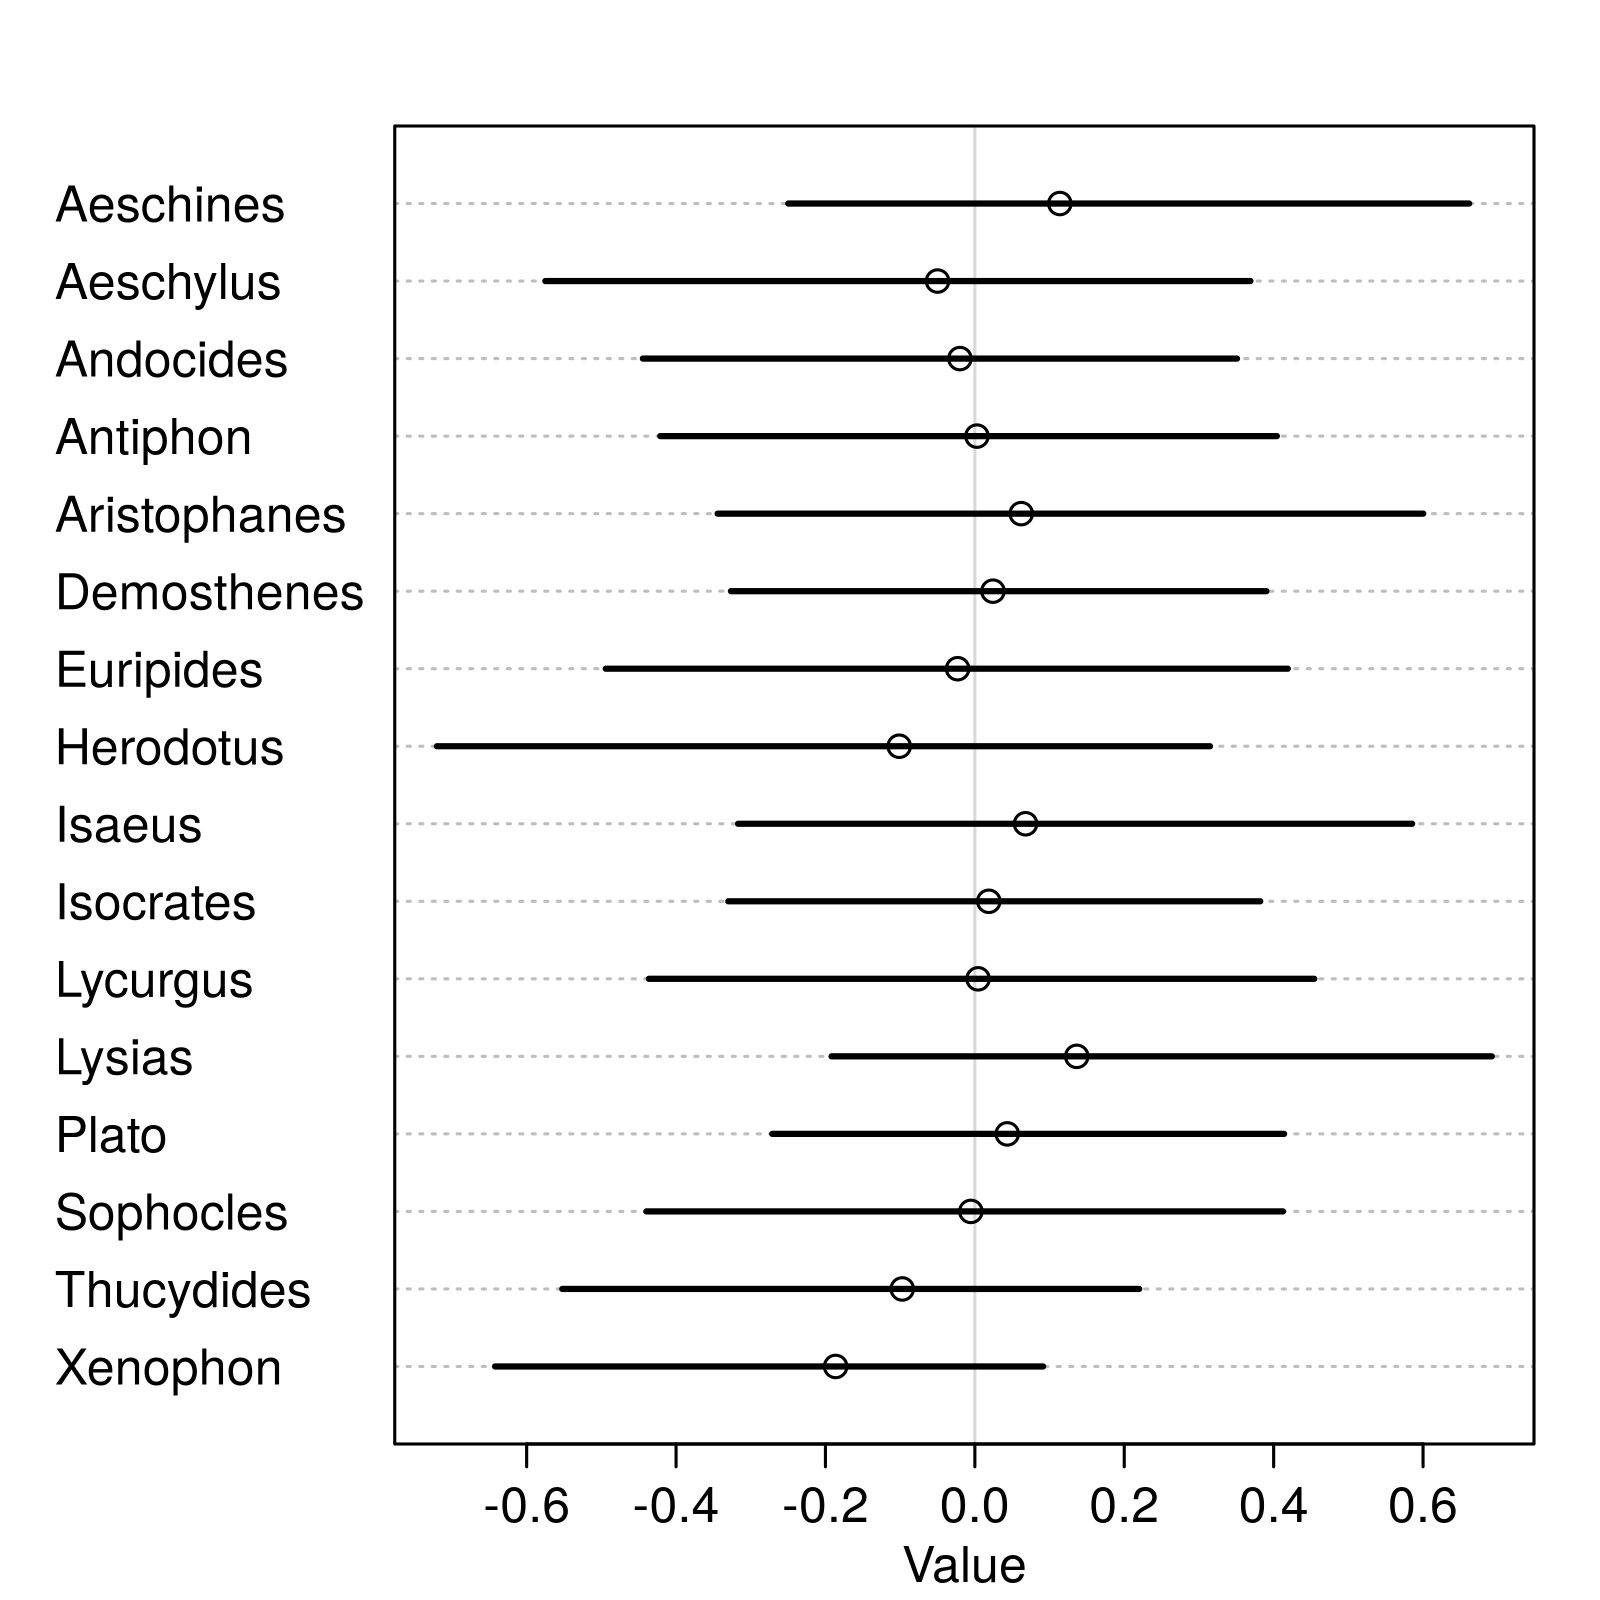
\includegraphics[width=0.75\linewidth]{../analysis/figs/precis_author.png}
\end{center}


\renewcommand*{\mkbibnamefamily}[1]{\textsc{#1}}
\printbibliography%
\renewcommand*{\mkbibnamefamily}[1]{#1}

\end{document}
